\documentclass{report}\usepackage[]{graphicx}\usepackage[]{color}
%% maxwidth is the original width if it is less than linewidth
%% otherwise use linewidth (to make sure the graphics do not exceed the margin)
\makeatletter
\def\maxwidth{ %
  \ifdim\Gin@nat@width>\linewidth
    \linewidth
  \else
    \Gin@nat@width
  \fi
}
\makeatother

\definecolor{fgcolor}{rgb}{0.345, 0.345, 0.345}
\newcommand{\hlnum}[1]{\textcolor[rgb]{0.686,0.059,0.569}{#1}}%
\newcommand{\hlstr}[1]{\textcolor[rgb]{0.192,0.494,0.8}{#1}}%
\newcommand{\hlcom}[1]{\textcolor[rgb]{0.678,0.584,0.686}{\textit{#1}}}%
\newcommand{\hlopt}[1]{\textcolor[rgb]{0,0,0}{#1}}%
\newcommand{\hlstd}[1]{\textcolor[rgb]{0.345,0.345,0.345}{#1}}%
\newcommand{\hlkwa}[1]{\textcolor[rgb]{0.161,0.373,0.58}{\textbf{#1}}}%
\newcommand{\hlkwb}[1]{\textcolor[rgb]{0.69,0.353,0.396}{#1}}%
\newcommand{\hlkwc}[1]{\textcolor[rgb]{0.333,0.667,0.333}{#1}}%
\newcommand{\hlkwd}[1]{\textcolor[rgb]{0.737,0.353,0.396}{\textbf{#1}}}%

\usepackage{framed}
\makeatletter
\newenvironment{kframe}{%
 \def\at@end@of@kframe{}%
 \ifinner\ifhmode%
  \def\at@end@of@kframe{\end{minipage}}%
  \begin{minipage}{\columnwidth}%
 \fi\fi%
 \def\FrameCommand##1{\hskip\@totalleftmargin \hskip-\fboxsep
 \colorbox{shadecolor}{##1}\hskip-\fboxsep
     % There is no \\@totalrightmargin, so:
     \hskip-\linewidth \hskip-\@totalleftmargin \hskip\columnwidth}%
 \MakeFramed {\advance\hsize-\width
   \@totalleftmargin\z@ \linewidth\hsize
   \@setminipage}}%
 {\par\unskip\endMakeFramed%
 \at@end@of@kframe}
\makeatother

\definecolor{shadecolor}{rgb}{.97, .97, .97}
\definecolor{messagecolor}{rgb}{0, 0, 0}
\definecolor{warningcolor}{rgb}{1, 0, 1}
\definecolor{errorcolor}{rgb}{1, 0, 0}
\newenvironment{knitrout}{}{} % an empty environment to be redefined in TeX

\usepackage{alltt}
\usepackage{geometry}
\geometry{a4paper,textwidth=15.92cm,textheight=24.62cm}
\usepackage{verbatim}
\usepackage{rotating}
\usepackage{lscape}
\usepackage{hyperref}
\usepackage[T1]{fontenc}
%\usepackage[nodayofweek]{datetime}
\usepackage[ddmmyy]{datetime}
\usepackage{enumitem}
\usepackage{setspace}
\usepackage{graphicx,wrapfig,lipsum}
\usepackage{fancyhdr}

\makeatletter
\newcommand{\verbatimfont}[1]{\def\verbatim@font{#1}}%
\makeatother

% following to define a new section style that takes less space
\makeatletter % make "at" ("@") letter, important for the code that follows
\renewcommand\chapter{\@startsection%
{chapter}{1}{0pt}%name, level, indent
{-\baselineskip}%beforeskip
{0.2\baselineskip}%afterskip
{\raggedright\bf}}%
\makeatother

\makeatletter
\renewcommand\section{\@startsection%
{section}{2}{0pt}%name, level, indent
{-\baselineskip}%beforeskip
{0.2\baselineskip}%afterskip
{\raggedright\bf}}%
\makeatother

\makeatletter
\setlength{\@fptop}{0pt}
\makeatother

\setlength{\tabcolsep}{3pt}
\setlength{\parskip}{1em}
\renewcommand*\contentsname{Table of contents}

\newcommand{\MONTH}{%
  \ifcase\the\month
  \or January
  \or February
  \or March
  \or April
  \or May
  \or June
  \or July
  \or August
  \or September
  \or October
  \or November
  \or December
  \fi}

\renewcommand{\dateseparator}{}

%\definecolor{red}{rgb}{0.8,0,0}
%\definecolor{yellow}{rgb}{0.8,0.8,0}
\definecolor{green}{rgb}{0,0.8,0}
\definecolor{gray}{rgb}{0.5,0.5,0.5}

\pagestyle{fancy}
\fancyhf{}
\fancyhead[L]{\textcolor{gray}{THE NATURE CONSERVANCY INDONESIA FISHERIES CONSERVATION PROGRAM \\ AR\_712713\_{\today}}}
\rfoot{\thepage}
\IfFileExists{upquote.sty}{\usepackage{upquote}}{}
\begin{document}
% use "echo=False" to remove R code from the output


\newgeometry{left=1cm,top=1cm,right=1cm,bottom=1cm}
\begin{titlepage}
\begin{flushleft}
	\textsf{Report Code: AR\_GROUPER\_{\today}}
\end{flushleft}

\vspace*{2cm}
\begin{flushright}
        {\Large\textsf{Length-Based Assessment of Data-Poor Multi-Species Deep Grouper Fisheries in 
        \\[0.2cm] Fisheries Management Areas (WPP) 573, 712, 713, 714, 715 \& 718 in Indonesia}}\\[0.2cm]
        \rule{\linewidth}{0.5mm}
        \textsf{DRAFT - NOT FOR DISTRIBUTION. TNC-IFCP Technical Paper}\\[2cm]
        \textsf{Peter J. Mous, Jos S. Pet\\[1cm]
        {\MakeUppercase{\MONTH}} {\the\day}, {\the\year}}
\end{flushright}

\begin{center}
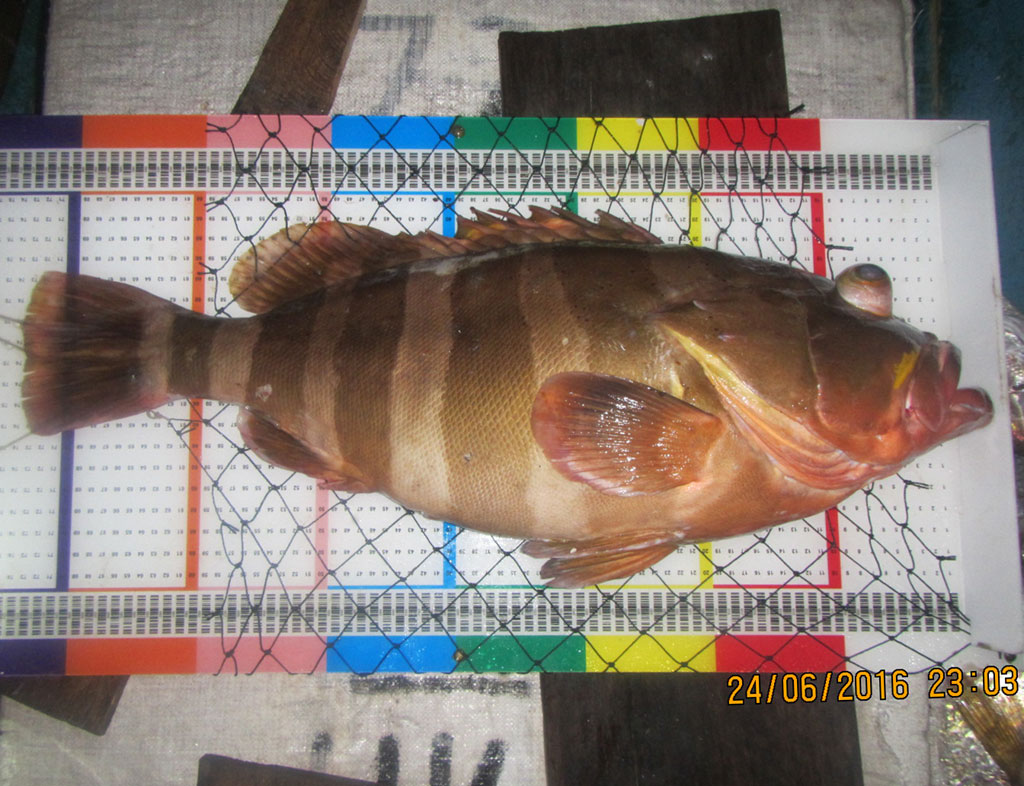
\includegraphics[width=.9\linewidth]{/root/R-project/IFishGrouper/Images/cover_ifish_grouper.jpg}
\end{center}

\vfill

\noindent
\begin{minipage}[b]{\linewidth}
\noindent
\centering
$\vcenter{\hbox{
\includegraphics[width=.3\linewidth]{/root/R-project/IFishGrouper/Images/usaid.png}}}$
\hfill
$\vcenter{\hbox{
\includegraphics[width=.3\linewidth]{/root/R-project/IFishGrouper/Images/tnc.png}}}$
\hfill
$\vcenter{\hbox{
\includegraphics[width=.3\linewidth]{/root/R-project/IFishGrouper/Images/pnci.png}}}$
\end{minipage}
\end{titlepage}
\restoregeometry

\vspace*{\fill}
\begin{sffamily}
\noindent\large For inquiries, please contact Dr. Peter Mous at pmous@tnc.org or Dr. Jos Pet at pet.jos@gmail.com\\
\end{sffamily}

\noindent
\fbox{\begin{minipage}[b]{\linewidth}
\begin{sffamily}
\begin{spacing}{0.4}
\textbf{The Nature Conservancy Indonesia Fisheries Conservation Program}\\[0.1cm]
Jl. Pura Segara, Pelabuhan Raya Benoa\\
Denpasar 3012\\
Bali, Indonesia\\
Ph. +62-361-244524, fax +62-361-244532\\[1cm]

\textbf{People and Nature Consulting International}\\[0.1cm]
Grahalia Tiying Gading 18, Suite 2\\
Jalan Tukad Pancoran, Panjer\\
Denpasar 80225
Bali, Indonesia\\
Ph. +62-361-257246\\
\end{spacing}
\end{sffamily}
\end{minipage}}
\clearpage

\tableofcontents

\vfill

\large

\chapter{Introduction}
This report presents a length-based assessment of the multi-species deep slope fisheries targeting mostly snappers, groupers and emperors, at depths ranging from 50 to 500 meters, in fisheries management areas (WPP) 714 and 715 in eastern Indonesia. These WPPs cover the Maluku, Seram, Banda and Flores Seas and they were combined as a single area for analysis, as the border between WPP 714 and WPP 715 cuts through the middle of the fishing grounds. Drop line and mini long line vessels fish on both sides of this border sometimes even within a single fishing trip. Also in terms of habitat and ecology of the target species the 2 WPPs covered in this report are very similar and completely connected. Fishing grounds for snappers, groupers, emperors and other target species in this region include deep slopes along the many islands as well as seamounts and other deep structures which are characteristic for this area.

Several fleets from this region contributed data to the current assessment, including a medium scale drop line fishery based in Kema (20 boats), North Sulawesi, and a small scale mini long line fishery based in the Banggai and Sula Islands on the border of the Maluku and Banda Seas. In addition, data were used from fleets originating from outside the region (e.g. Bali, Probolinggo, Kupang) but operating inside WPP 714 and/or WPP715. Fishing grounds for the small scale mini long line fleet are concentrated near the home islands near the center of our area of interest, whereas the medium scale drop liners from Kema make trips to locations up to 1,000 kilometers away from their port, to all corners of this region.

Kema based vessels make up to about 10 trips a year, landing around 4 tons of mixed snapper, grouper and emperor for each trip or up to about 40 tons per vessel per year. The drop line fishery is an active vertical hook and line fishery operating at depths from 50 to 500 meters, whereas long lines are set horizontally along the bottom at depths ranging from 50 to 150 meters. This report analyzes length frequencies of the 50 species of fish that were the most abundant in the combined drop and long line fisheries operating in WPP 714 and WPP 715. For a complete overview of the species composition please refer to the ID guide prepared for these fisheries:

\textbf{CLICK: }\href{http://72.14.187.103:8080/ifish/pub/TNC_FishID.pdf}{Link to on-line E-Book Species ID Guide}

For further background on species life history characteristics, and data-poor length based assessment methods, as applied in this report, please refer to the assessment guide that was separately prepared for these fisheries:

\textbf{CLICK: }\href{http://72.14.187.103:8080/ifish/pub/DeepSlopeSpeciesAssessmentTool.pdf}{Link to on-line E-Book Assessment Guide with Biological Information}

Data in this report represent complete catches by small and medium scale vessels from the above described fleets. All fish captured were photographed on measuring boards by fishing crew participating in our Crew Operated Data Recording System or CODRS. Images were analyzed by project staff to generate the species specific length frequency distributions of the catches which served as the input for our length based assessment of this fishery.

\begin{center}
\graphicspath{{/root/R-project/IFishSnapperWPP714_715/Images/}}
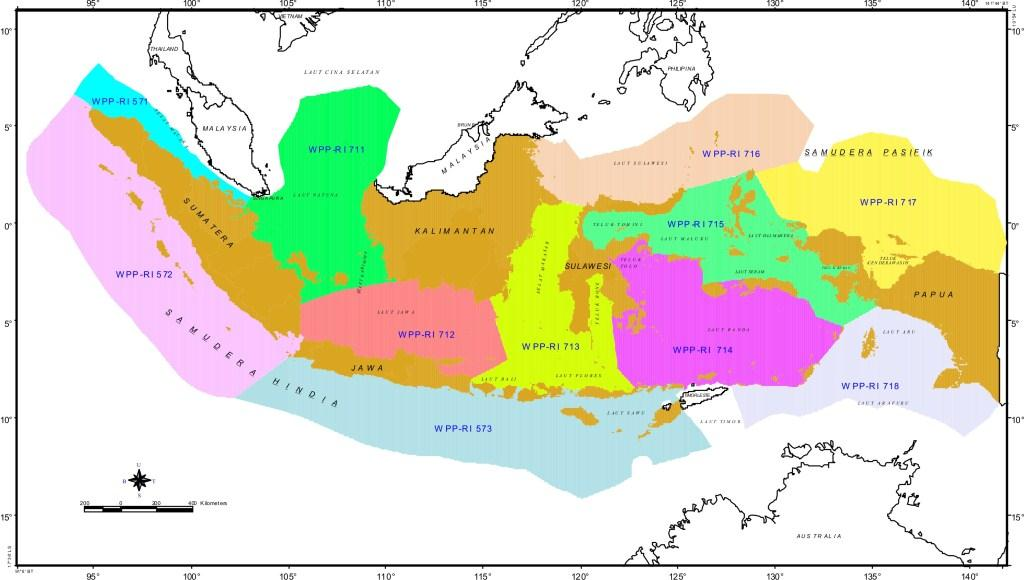
\includegraphics[scale=1.8]{wpp-indonesia.jpg}

Figure 1. Fisheries Management Areas (WPP) in Indonesian marine waters.
\end{center}

\begin{center}
\graphicspath{{/root/R-project/IFishSnapperWPP714_715/Images/}}
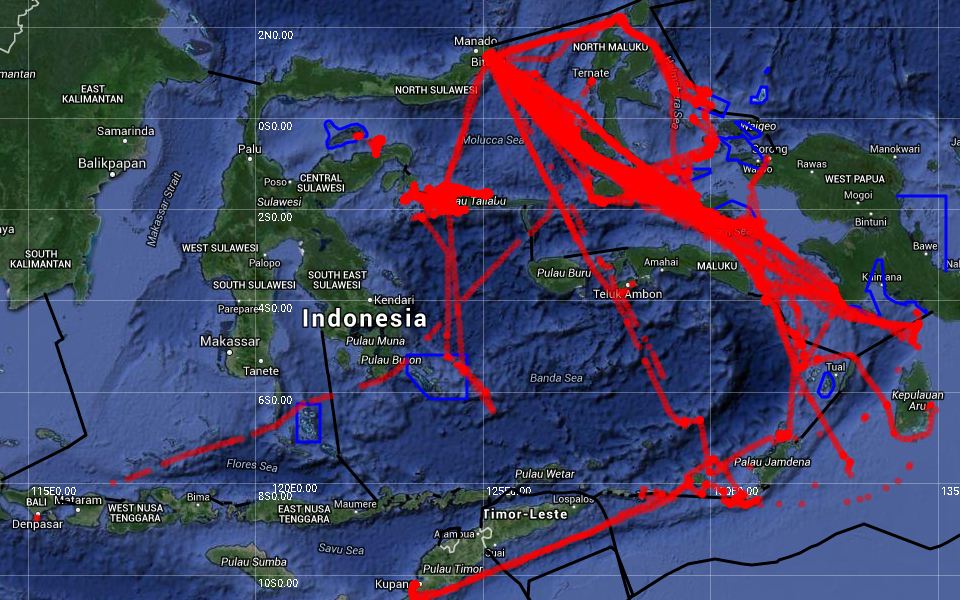
\includegraphics[scale=0.6]{SpotTrace-AreaC-Satellite.jpg}

Figure 2. Map with fishing ground bathymetry and tracks (in red) of snapper fishing trips into WPP 714 and 715. Black lines are WPP boundaries, blue lines are MPA boundaries. This figure mainly represents fleets from Kema (near Manado) and the Banggai / Sula Islands.
\end{center}

% latex table generated in R 3.2.2 by xtable 1.7-4 package
% Mon Feb 20 06:12:50 2017
\begin{table}[ht]
\centering
\caption{Sample Sizes, Length-Weight Relationships \& Trading Limits Snapper Fisheries Indonesia} 
{\small
\begin{tabular}{ccccccccccc}
  \hline
 &  & Reported &  &  & Length & Converted & Plotted &  &  &  \\ 
  { } & { } & {Trade} & \multicolumn{2}{c}{ W = a L\textsuperscript{b}} & {Type} & {Trade} & {Trade} & \multicolumn{3}{c}{Sample Size}\\
      { } & { } & {Limit} & { } & { } & {for a \& b} & {Limit} & {Limit} & { } & { } & { }\\
      {\#ID} & {Species} & {Weight (g)} & {a} & {b} & {TL-FL-SL} & {L(cm)} & {TL(cm)} & {2015} & {2016} & {2017}\\ \hline
1 & Aphareus rutilans & 1000 & 0.015 & 2.961 & FL & 42.20 & 49.61 & 0 & 19 & 2 \\ 
  2 & Aprion virescens & 1000 & 0.023 & 2.886 & FL & 40.49 & 45.90 & 0 & 119 & 11 \\ 
  7 & Pristipomoides multidens & 500 & 0.020 & 2.944 & FL & 31.18 & 34.92 & 0 & 19934 & 772 \\ 
  8 & Pristipomoides typus & 500 & 0.014 & 2.916 & TL & 36.16 & 36.16 & 0 & 2690 & 202 \\ 
  9 & Pristipomoides filamentosus & 500 & 0.038 & 2.796 & FL & 29.70 & 33.27 & 0 & 176 & 0 \\ 
  16 & Lutjanus argentimaculatus & 500 & 0.034 & 2.792 & FL & 31.22 & 31.78 & 0 & 93 & 7 \\ 
  17 & Lutjanus bohar & 500 & 0.016 & 3.059 & FL & 29.70 & 31.31 & 0 & 117 & 4 \\ 
  18 & Lutjanus malabaricus & 500 & 0.009 & 3.137 & FL & 33.11 & 33.11 & 0 & 4979 & 867 \\ 
  19 & Lutjanus sebae & 500 & 0.009 & 3.208 & FL & 29.97 & 31.26 & 0 & 1157 & 46 \\ 
  20 & Lutjanus timorensis & 500 & 0.009 & 3.137 & FL & 33.11 & 33.34 & 0 & 619 & 29 \\ 
  21 & Lutjanus gibbus & 500 & 0.015 & 3.091 & FL & 28.87 & 31.09 & 0 & 33 & 0 \\ 
  22 & Lutjanus erythropterus & 500 & 0.024 & 2.870 & FL & 31.79 & 31.79 & 0 & 90 & 4 \\ 
  25 & Lutjanus russelli & 300 & 0.020 & 2.907 & FL & 27.28 & 28.49 & 0 & 47 & 2 \\ 
  27 & Lutjanus vitta & 300 & 0.017 & 2.978 & FL & 26.72 & 27.64 & 0 & 1819 & 16 \\ 
  28 & Lutjanus boutton & 300 & 0.034 & 3.000 & FL & 20.75 & 21.56 & 0 & 70 & 0 \\ 
  31 & Symphorus nematophorus & 1000 & 0.015 & 3.046 & FL & 38.63 & 40.18 & 0 & 176 & 22 \\ 
  39 & Cephalopholis sonnerati & 300 & 0.015 & 3.058 & TL & 25.78 & 25.78 & 0 & 518 & 6 \\ 
  41 & Epinephelus latifasciatus & 1500 & 0.010 & 3.088 & TL & 48.00 & 48.00 & 0 & 147 & 18 \\ 
  43 & Epinephelus morrhua & 300 & 0.061 & 2.624 & FL & 25.59 & 25.59 & 0 & 44 & 1 \\ 
  44 & Epinephelus poecilonotus & 500 & 0.061 & 2.624 & FL & 31.09 & 31.09 & 0 & 18 & 1 \\ 
  45 & Epinephelus areolatus & 300 & 0.011 & 3.048 & FL & 28.18 & 28.77 & 0 & 9390 & 18 \\ 
  46 & Epinephelus bleekeri & 300 & 0.009 & 3.126 & TL & 28.09 & 28.09 & 0 & 70 & 8 \\ 
  49 & Epinephelus malabaricus & 1500 & 0.013 & 3.034 & TL & 46.85 & 46.85 & 0 & 14 & 2 \\ 
  50 & Epinephelus coioides & 1500 & 0.011 & 3.084 & TL & 46.94 & 46.94 & 0 & 21 & 2 \\ 
  53 & Epinephelus heniochus & 300 & 0.061 & 2.624 & FL & 25.59 & 25.59 & 0 & 552 & 7 \\ 
  55 & Epinephelus epistictus & 1500 & 0.009 & 3.126 & TL & 47.01 & 47.01 & 0 & 49 & 0 \\ 
  58 & Epinephelus amblycephalus & 1500 & 0.012 & 3.057 & TL & 45.99 & 45.99 & 0 & 150 & 16 \\ 
  61 & Plectropomus leopardus & 500 & 0.012 & 3.060 & FL & 32.56 & 33.38 & 0 & 242 & 9 \\ 
  62 & Variola albimarginata & 300 & 0.012 & 3.079 & FL & 26.68 & 30.44 & 0 & 44 & 2 \\ 
  63 & Lethrinus erythracanthus & 500 & 0.032 & 2.885 & FL & 28.43 & 29.56 & 0 & 42 & 0 \\ 
  65 & Lethrinus lentjan & 300 & 0.020 & 2.986 & FL & 25.16 & 26.35 & 0 & 245 & 4 \\ 
  67 & Lethrinus olivaceus & 300 & 0.029 & 2.851 & FL & 25.49 & 27.50 & 0 & 176 & 31 \\ 
  68 & Lethrinus amboinensis & 300 & 0.029 & 2.851 & FL & 25.49 & 28.06 & 0 & 63 & 0 \\ 
  70 & Wattsia mossambica & 500 & 0.040 & 2.824 & FL & 28.21 & 29.34 & 0 & 13 & 0 \\ 
  71 & Gymnocranius grandoculis & 500 & 0.032 & 2.885 & FL & 28.43 & 30.53 & 0 & 1417 & 45 \\ 
  72 & Gymnocranius griseus & 500 & 0.032 & 2.885 & FL & 28.43 & 30.56 & 0 & 371 & 3 \\ 
  74 & Carangoides fulvoguttatus & 1000 & 0.033 & 2.808 & FL & 39.51 & 43.62 & 0 & 51 & 1 \\ 
  76 & Carangoides chrysophrys & 1000 & 0.027 & 2.902 & FL & 37.68 & 42.12 & 0 & 93 & 8 \\ 
  77 & Carangoides gymnostethus & 1000 & 0.046 & 2.746 & FL & 37.88 & 41.55 & 0 & 22 & 0 \\ 
  78 & Caranx ignobilis & 2000 & 0.027 & 2.913 & FL & 46.78 & 54.36 & 0 & 54 & 4 \\ 
  80 & Caranx sexfasciatus & 2000 & 0.032 & 2.930 & FL & 43.43 & 49.51 & 0 & 14 & 0 \\ 
  81 & Caranx tille & 2000 & 0.032 & 2.930 & FL & 43.43 & 49.51 & 0 & 35 & 1 \\ 
  83 & Seriola dumerili & 2000 & 0.022 & 2.847 & TL & 54.74 & 54.74 & 0 & 32 & 10 \\ 
  84 & Seriola rivoliana & 2000 & 0.006 & 3.170 & FL & 54.23 & 60.03 & 0 & 33 & 0 \\ 
  86 & Argyrops spinifer & 300 & 0.055 & 2.670 & TL & 25.11 & 27.87 & 0 & 136 & 3 \\ 
  88 & Glaucosoma buergeri & 500 & 0.045 & 2.725 & TL & 30.40 & 30.40 & 0 & 41 & 0 \\ 
  90 & Diagramma pictum & 500 & 0.014 & 2.988 & FL & 33.08 & 36.71 & 0 & 559 & 34 \\ 
  96 & Ostichthys japonicus & 300 & 0.018 & 3.020 & FL & 25.10 & 26.23 & 0 & 142 & 1 \\ 
  97 & Rachycentron canadum & 1000 & 0.003 & 3.088 & FL & 60.67 & 67.28 & 0 & 79 & 2 \\ 
  100 & Branchiostegus australiensis & 1000 & 0.010 & 3.040 & FL & 44.13 & 44.13 & 0 & 26 & 0 \\ 
   \hline
\end{tabular}
}
\end{table}


\clearpage
\newpage

\chapter{Materials and methods for data collection, analysis and reporting}
\section{SPOT Trace vessel tracking}

Fishing grounds are determined by deploying Spot Trace units on various fishing boats. When in motion, Spot Trace units automatically report an hourly location, and when at rest for more than 24 hours, they relay daily status reports. Location and status report messages are automatically recorded in I-Fish Community, an online database running PostgreSQL with a user interface programmed in Java and analysis and reporting procedures in R and Latex.

Fishing vessels with Spot Trace units on board generate accurate data on fishing grounds and specific fishing locations within fishing grounds. Traditionally, fishing ground data were often collected from logbook data or captain interviews. However, logbook and interview data are sometimes unclear, inaccurate and can easily be tampered with. Spot Trace enables us to match catch data with exact fishing locations, while providing additional safety for the fishing vessels. To mitigate IUU fishing accusations, having the Spot Trace onboard can also be used as proof of legal fishing within Indonesian waters.


\section{Crew Operated Data Recording System}

Data on species and size distributions of complete catches are needed for accurate length based stock assessments. Such data on individual fishing trips are collected via Crew Operated Data Recording Systems or CODRS. This catch data is geo-referenced as the CODRS works in tandem with the Spot Trace vessel tracking system. Crews of fishing vessels are contracted to take images on project-supplied digital cameras of all fish in the catch, positioned over measuring boards. This procedure takes place when batches of fish are taken from chiller boxes on deck, before they are packed on ice in the hold. The crew photographs all the fish in this manner and at the end of the trip hands in the storage chip from the camera to a project stage who analysis the images back at the fisheries station. Double checking with owner and trader data on total catches, and comparison with weights as calculated from fish lengths, showed that we were indeed capturing length frequencies of most if not all fish in the catch in this manner. No species or size classes were missing before analysis.

Analysis of the CODRS images includes ID of the species and reading of the length of the fish as displayed on the measuring board. The image analysis is done by highly trained and experienced project stage and interns, based at our fisheries stations. Data processing, analysis and reporting are done through I-Fish Community, which also receives data on fishing grounds via the Spot Trace units deployed on fishing vessels. All data are stored in real time in the I-Fish Community database, where it is aggregated and analyzed with length-based methods.

\clearpage
\newpage

\section{Smart Weighing and Measuring System}

As part of a land-based traceability and monitoring approach, data collection on species specific size distributions was also done through a smart weighing and measuring system (SWMS) for fish processed at mini plants. The SWMS collects complete and detailed information on traded fish species, length and weight, for every single fish that is received and processed by the company. The SWMS is inserted seamlessly into the production line to minimize interference with the pre-existing workflow. In addition to data collection, the SWMS also allows companies to use the system to do internal auditing on production and orders, and to generate invoices for different suppliers.

The smart weighing scale system comprises of hardware (touch screen computers connected to digital scales, measuring board, scanners and barcode printers) and software (integrated traceability and data collection software that is used for business intelligence provided by Insite Solutions, a US-based IT company). Length of individual fish is measured using a bar-coded measuring board-with a barcode at every one-centimeter mark. Personnel of the processing plant position the  sh on a bar-coded measuring board, and they scan the barcode where the fish tail ends (total length). Length data is then automatically recorded in the database on a server, and from there transferred to I-Fish Community.


\section{I-Fish Community}

I-Fish Community only stores data that are relevant to fisheries management, whereas data on processed volume and sales, from the Smart Weighing and Measuring System, remain on servers at processing companies. Access to the I-Fish Community database is controlled by user name and password. I-Fish Community has different layers of privacy, which is contingent on the user's role in the supply chain. For instance, boat owners may view exact location of their boats, but not of the boats of other owners.

I-Fish Community has an automatic length-frequency distribution reporting system for length-based assessment of the fishery by species. The database generates length frequency distribution graphs for each species, together with life history parameters including length at maturity (Lmat), optimum harvest size (Lopt), asymptotic length- (Linf), and maximum total length (Lmax), as well as size limits used in the trade. These "trade limit" lengths are derived from general buying behavior (minimal weight) of processing companies. The weights are converted into lengths by using species-specific length- weight relationships.

Each length frequency distribution is accompanied by an automated length-based assessment on current status of the fishery by species. Any I-Fish Community user can access these graphs and the conclusions from the assessments. The report produces an assessment for the 50 most abundant species in the fishery, based on complete catches from the most recent complete calendar year (to ensure full year data sets). The graphs show the position of the catch length frequency distributions relative to various life history parameter values and trading limits for each species. Relative abundance of specific size groups is plotted for all years for which data are available, to indicate trends in status by species.

\clearpage
\newpage

Immature fish, small mature fish, large mature fish, and a subset of large mature fish, namely "mega-spawners", which are fish larger than 1.1 times the optimum harvest size (Froese 2004), make up the specific size groups used in our length based assessment. For all fish of each species in the catch, the percentage in each category is calculated for further use in the length based assessment. These percentages are calculated and presented as the first step in the length based assessment as follows: W\% is immature (smaller than the length at maturity), X\% is small matures (at or above size at maturity but smaller than the optimum harvest size), and Y\% is large mature fish (at or above optimum harvest size). The percentage of mega-spawners is Z\%.

The automated assessment comprises of six elements from the catch length frequencies. These elements all work with length based indicators of various kinds to draw conclusions from species specific length frequencies in the catch.

\textit{1. Proportion of immature fish in the catch.}

With 0\% immature fish in the catch as an ideal target (Froese, 2004), a target of 10\% or less is considered a reasonable indicator for sustainable (or safe) harvesting (Fujita et al., 2012; Vasilakopoulos et al., 2011). Zhang et al. (2009) consider 20\% immature fish in the catch as an indicator for a fishery at risk, in their approach to an ecosystem based fisheries assessment. Results from meta-analysis over multiple fisheries showed stock status over a range of stocks to fall below precautionary limits at 30\% or more immature fish in the catch (Vasilakopoulos et al., 2011). The fishery is considered highly at risk when more than 50\% of the fish in the catch are immature (Froese et al, 2016).

IF "\% immature" is lower than or equal to 10\% THEN:\\[0cm]
"At least 90\% of the fish in the catch are mature specimens that have spawned at least once before they were caught. The fishery does not depend on immature size classes for this species and is considered safe for this indicator. This fishery will not be causing overfishing through over harvesting of juveniles for this species. Risk level is low."

ELSE, IF "\% immature" is greater than 10\% AND "\% immature" is lower than or equal to 20\% THEN:\\[0cm]
"Between 10\% and 20\% of the fish in the catch are juveniles that have not yet reproduced. There is no immediate concern in terms of overfishing through over harvesting of juveniles, but the fishery needs to be monitored closely for any further increase in this indicator and incentives need to be geared towards targeting larger fish. Risk level is medium."

ELSE, IF "\% immature" is greater than 20\% AND "\% immature" is lower than or equal to 30\% THEN:\\[0cm]
"Between 20\% and 30\% of the fish in the catch are specimens that have not yet reproduced. This is reason for concern in terms of potential overfishing through overharvesting of juveniles, if fishing pressure is high and percentages immature fish would further rise. Targeting larger fish and avoiding small fish in the catch will promote a sustainable fishery. Risk level is medium."

\clearpage
\newpage

ELSE, IF "\% immature" is greater than 30\% AND "\% immature" is lower than or equal to 50\% THEN:\\[0cm]
"Between 30\% and 50\% of the fish in the catch are immature and have not had a chance to reproduce before capture. The fishery is in immediate danger of overfishing through overharvesting of juveniles, if fishing pressure is high.  Catching small and immature fish needs to be actively avoided and a limit on overall fishing pressure is warranted. Risk level is high."

ELSE, IF "\% immature" is greater than 50\% THEN:\\[0cm]
"The majority of the fish in the catch have not had a chance to reproduce before capture. This fishery is most likely overfished already if fishing mortality is high for all size classes in the population. An immediate shift away from targeting juvenile fish and a reduction in overall fishing pressure is essential to prevent collapse of the stock. Risk level is high."

\textit{2. Minimum size as traded compared to length and maturity.}

We use a comparison between the trade limit (minimum size accepted by the trade) and the size at maturity as an indicator for incentives from the trade for either unsustainable targeting of juveniles or for more sustainable targeting of mature fish that have spawned at least once. We consider a trade limit at 10\% below or above the length at maturity to be significantly different from the length at maturity and we consider trade limits to provide incentives for targeting of specific sizes of fish through price differentiation.

IF "TradeLimit" is lower than 0.9 * L-mat THEN:\\[0cm]
"The trade limit is significantly lower than the length at first maturity.  This means that the trade encourages capture of immature fish, which impairs sustainability. Risk level is high."

ELSE, IF "TradeLimit" is greater than or equal to 0.9 * L-mat AND "TradeLimit" is lower than or equal to 1.1 * L-mat THEN:\\[0cm]
"The trade limit is about the same as the length at first maturity.  This means that the trade puts a premium on fish that have spawned at least once, which improves sustainability of the fishery. Risk level is medium."

ELSE, IF "TradeLimit" is greater than 1.1 * L-mat THEN:\\[0cm]
"The trade limit is significantly higher than length at first maturity.  This means that the trade puts a premium on fish that have spawned at least once. The trade does not cause any concern of recruitment overfishing for this species. Risk level is low."

\textit{3. Current exploitation level.}

We use the current exploitation level expressed as the percentage of fish in the catch below the optimum harvest size as an indicator for fisheries status. We consider a proportion of 65\% of the fish (i.e. the vast majority in numbers) in the catch below the optimum harvest size as an indicator for growth overfishing. We also consider a majority in the catch around or above the optimum harvest size as an indicator for minimizing the impact of fishing (Froese et al., 2016). This indicator will be achieved when less than 50\% of the fish in the catch are below the optimum harvest size.

\clearpage
\newpage

IF "\% immature + \% small mature" is greater than or equal to 65\% THEN:\\[0cm]
"The vast majority of the fish in the catch have not yet achieved their growth potential. The harvest of small fish promotes growth overfishing and the size distribution for this species indicates that over exploitation through growth overfishing may already be happening. Risk level is high."

ELSE, IF "\% immature + \% small mature" is lower than or equal to 50\% THEN:\\[0cm]
"The majority of the catch consists of size classes around or above the optimum harvest size. This means that the impact of the fishery is minimized for this species. Potentially higher yields of this species could be achieved by catching them at somewhat smaller size, although capture of smaller specimen may take place already in other fisheries. Risk level is low."

ELSE, IF "\% immature + \% small mature" is greater than 50\% AND "\% immature + \% small mature" is lower than 65\% THEN:\\[0cm]
"The bulk of the catch includes age groups that have just matured and are about to achieve their full growth potential. This indicates that the fishery is probably at least being fully exploited. Risk level is medium."

\textit{4. Proportion of mega spawners in the catch.}

Mega spawners are fish larger than 1.1 times the optimum harvest size. We consider a proportion of 30\% or more mega spawners in the catch to be a sign of a healthy population (Froese, 2004), whereas lower proportions are increasingly leading to concerns, with proportions below 20\% indicating great risk to the fishery.

IF "\% mega spawners" is greater than 30\% THEN:\\[0cm]
"More than 30\% of the catch consists of mega spawners which indicates that this fish population is in good health unless large amounts of much smaller fish from the same population are caught by other fisheries. Risk level is low."

ELSE, IF "\% mega spawners" is greater than 20\% AND "\% mega spawners" is lower than or equal to 30\% THEN:\\[0cm]
"The percentage of mega spawners is between 20 and 30\%.  There is no immediate reason for concern, though fishing pressure may be significantly reducing the percentage of mega-spawners, which may negatively affect the reproductive output of this population. Risk level is medium."

ELSE, IF "\% mega spawners" is lower than or equal to 20\%, THEN:\\[0cm]
"Less than 20\% of the catch comprises of mega spawners.  This indicates that the population may be severely affected by the fishery, and that there is a substantial risk of recruitment overfishing through over harvesting of the mega spawners, unless large numbers of mega spawners would be surviving at other habitats. There is no reason to assume that this is the case and therefore a reduction of fishing effort may be necessary in this fishery. Risk level is high.

\clearpage
\newpage

\textit{5. Take less than nature.}

Rule number one to minimize the impact of fishing (Froese et al., 2016) teaches us to "take less than nature" by ensuring that mortality caused by fishing is less than the natural rate of mortality. We consider a fishing mortality of less than half the natural mortality to be necessary to minimize the impact of fishing. We estimated the instantaneous total mortality (Z) from the equilibrium Beverton-Holt estimator from length data using Ehrhardt and Ault (1992) bias-correction, implemented through the function bheq2 of the R Fishmethods package. We estimated the natural rate of mortality (M) using Froese and Pauly (2000) empirical formula with asymptotic length as estimated by species and an ambient water temperature at fishing depth estimated at about 20 degrees Celcius. With an asymptotic length for a snapper of about 80cm this results in an M of about 0.4, which aligns well with the mean of reported values from the literature (Martinez-Andrade, 2003). The fishing mortality F follows as the difference between total and natural mortality.

IF "fishing mortality" is greater than or equal to "natural mortality" THEN:\\[0cm]
Mortality caused by fishing is greater than or equal to the natural rate of mortality. This means that impact of fishing is severe and that fishing is unlikely to be sustainable at the current level of effort. Risk level is high.

IF "fishing mortality" is lower than "natural mortality" AND "fishing mortality" is greater than 0.5 times "natural mortality" THEN:\\[0cm]
Mortality caused by fishing is lower than the natural rate of mortality but more than half of natural mortality. This means that impact of fishing is considerable and trends in various indicators need to be watched carefully while any increase in fishing effort needs to be prevented. Risk level is medium.

IF "fishing mortality" is lower than or equal to 0.5 times "natural mortality" THEN:\\[0cm]
Mortality caused by fishing is at or below a level equal to half the natural rate of mortality. This means that impact of fishing is minimized and this fishery is currently probably operating at a sustainable level of effort. Risk level is low.

\textit{6. Spawning Potential Ratio.}

As an indicator for Spawning Potential Ratio (SPR, Quinn and Deriso, 1999), we used the estimated spawning stock biomass divided by the spawning stock biomass of that population it it would have been pristine (see, for example, Meester et al 2001). We calculated SPR on a per-recruit basis from life-history parameters Z, F, K (von Bertalanffy), and Linf. We estimated Z and F as explained above and K from Lopt, using the method presented in Froese and Binohlan 2000.

\clearpage
\newpage

In a perfect world, fishery biologists would know what the appropriate SPR should be for every harvested stock based on the biology of that stock. Generally, however, not enough is known about managed stocks to be so precise. However, studies show that some stocks (depending on the species of fish) can maintain themselves if the spawning stock biomass per recruit can be kept at 20 to 35\% (or more) of what it was in the un-fished stock. Lower values of SPR may lead to severe stock declines (Wallace and Fletcher, 2001). Froese et al. (2016) considered a total population biomass B of half the pristine population biomass Bo to be the lower limit reference point for stock size, minimizing the impact of fishing. Using SPR and B/Bo estimates from our own data set, this Froese et al. (2016) lower limit reference point correlates with an SPR of about 40\%, not far from but slightly more conservative than the Wallace and Fletcher (2001) reference point. We chose an SPR of 40\% as our reference point for high risk and after similar comparisons we consider and SPR between 25\% and 40\% to represent a medium risk situation.

IF "SPR" is lower than 25\% THEN:\\[0cm]
"SPR is less than 25\%. The fishery probably over-exploits the stock, and there is a substantial risk that the fishery will cause severe decline of the stock if fishing effort is not reduced. Risk level is high."

ELSE, IF "SPR" is greater than or equal to 25\% AND "SPR" is lower than 40\% THEN:\\[0cm]
"SPR is between 25\% and 40\%. The stock is heavily exploited, and there is some risk that the fishery will cause further decline of the stock. Risk level is medium."

ELSE, IF "SPR" is greater than or equal to 40\% THEN:\\[0cm]
"SPR is more than 40\%. The stock is probably not over exploited, and the risk that the fishery will cause further stock decline is small. Risk level is low."

\clearpage
\newpage

\begin{center}
\graphicspath{{/root/R-project/IFishGrouper/Images/}}
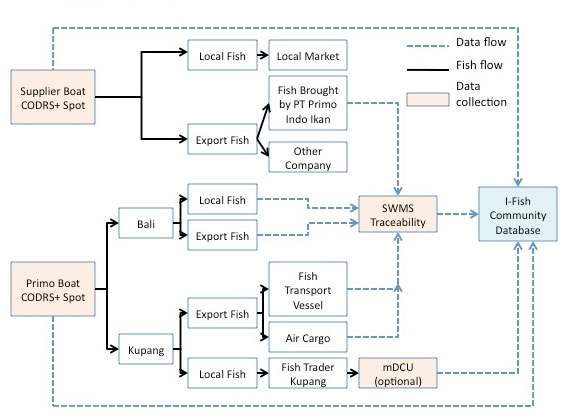
\includegraphics[scale=0.7]{supply_chain.jpg}

Figure 4. Example of the location of CODRS and SWMS within a single supply chain.
\end{center}

\begin{center}
\graphicspath{{/root/R-project/IFishGrouper/Images/}}
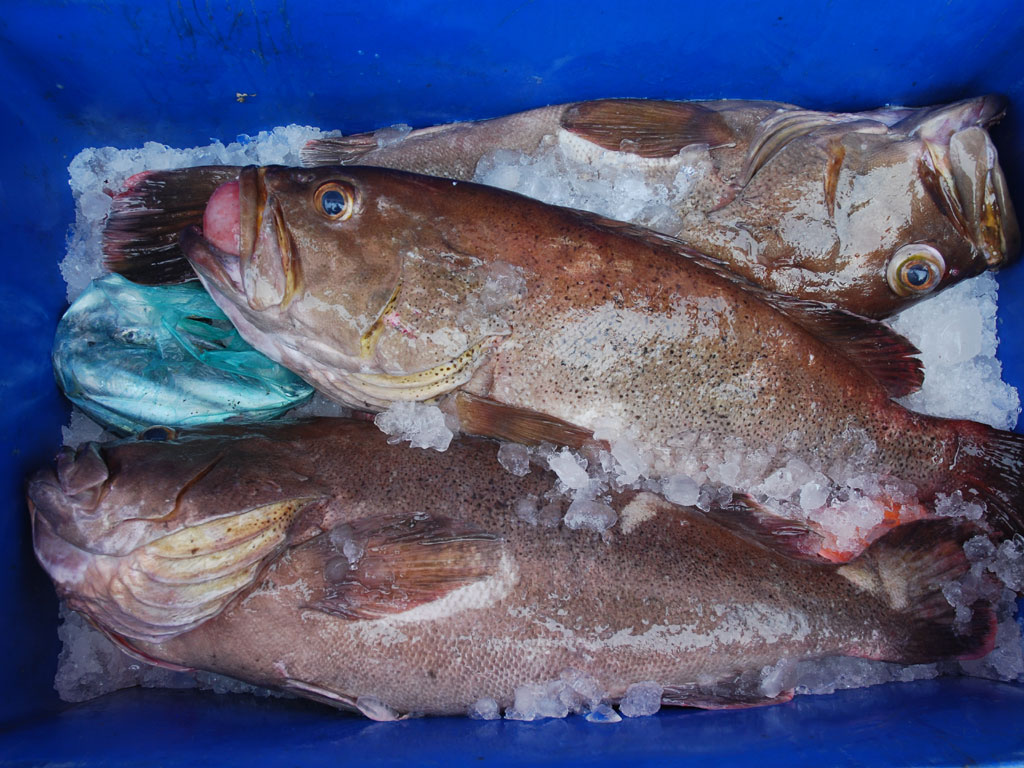
\includegraphics[scale=0.4]{groupers_delivered_to_a_trader.jpg}

Figure 5. Groupers (Epinephelus epistictus) delivered by a drop line fisher to a trader in South Lombok who supplies processors in Bali.
\end{center}

\newpage

\chapter{Fishing grounds and traceability}
The Spot Trace data from the Java Sea and Makassar Strait snapper fisheries illustrate that management by WPP is sometimes impossible. In the case of the snapper fisheries in WPP 712 and WPP 713, many vessels fish right at the border, often fishing in both these WPP even within single fishing trips. Also landings made at ports in any specific WPP, are not necessarily fish caught in that particular WPP, and this is especially true for snappers, groupers and emperors landed and processed in East Java, on the coast of WPP 712. The fish that is processed in major processing centers like Probolinggo comes from a number of different fleets that operate throughout the waters of Eastern Indonesian, including WPP 718 (Arafura Sea) and WPP 573 (Timor Sea).

\begin{center}
\graphicspath{{/root/R-project/IFishSnapperWPP712_713/Images/}}
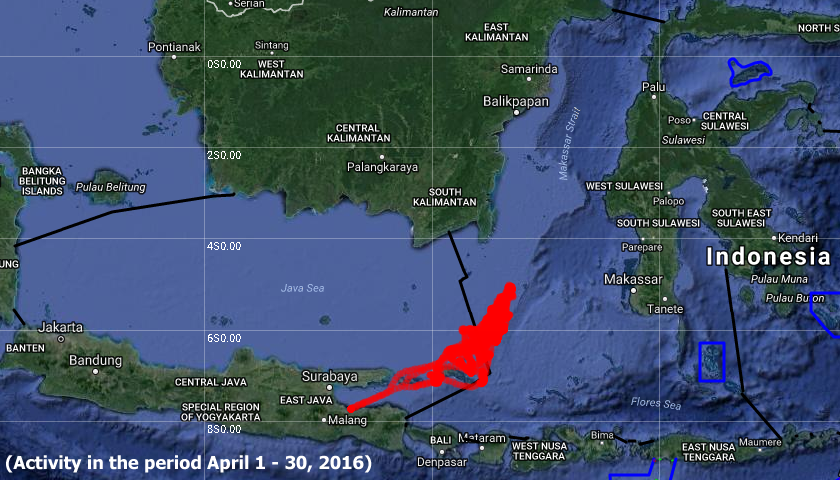
\includegraphics[width=15cm]{SpotTrace-712_713-April1-30_2016.png}

Figure 5. Tracks of long line and drop line fishing boats operating in the Java Sea (WPP 712) and the Makassar Strait (WPP 713).
\end{center}

\begin{center}
\graphicspath{{/root/R-project/IFishSnapperWPP712_713/Images/}}
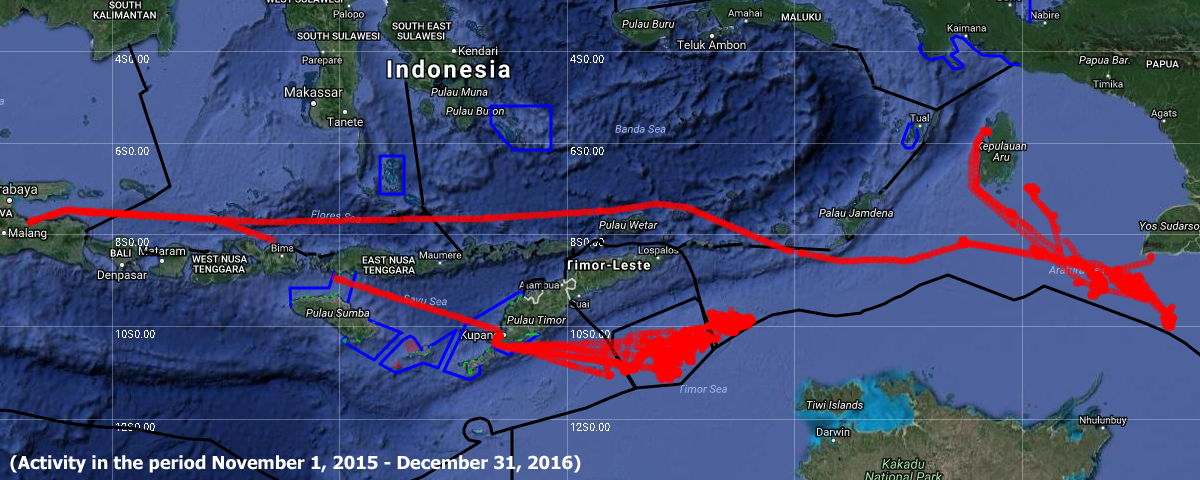
\includegraphics[width=15cm]{ProbolinggoFleetIn573_718_JPDA.png}

Figure 6. Tracks of long line fishing boats based in Probolingo, East Java, operating in the Timor Sea (WPP 573) and the Arafura Sea (WPP 718).
\end{center}


Potential IUU issues related to fish landed at ports in WPP 712 and 713 include the illegal operation by various fleets outside Indonesian waters in the East Timorese - Australian Joint Petroleum Development Area (JPDA). Fish from these waters may be mixed with fish from various Indonesian fisheries management areas, including WPP 712 and WPP 713, at the processing plants in Probolinggo. Additional issues include the under marking of medium scale vessels to below 30GT, the licensing of the various fleets for various WPP and the operation of fleets from remote ports inside Marine Protected Areas throughout Eastern Indonesia. All this needs to be discussed with fishing boat captains and boat owners to prevent issues of supply line ``pollution'' with IUU fish from thee protected areas.


\newpage

\chapter{Species-specific length-based assessments}
\verbatimfont{\normalfont\rmfamily}
\definecolor{fgcolor}{rgb}{0,0,0}
\begin{knitrout}
\definecolor{shadecolor}{rgb}{1, 1, 1}\color{fgcolor}
\includegraphics[width=\maxwidth]{/root/R-project/IFishSnapperWPP712_713/Plots/plot-LFD-1} 
\begin{kframe}\begin{verbatim}
\end{verbatim}
\end{kframe}
\clearpage
\newpage
\begin{kframe}\begin{verbatim}
The percentages of Aphareus rutilans (ID #1, Lutjanidae) in 2016, n = 19
Immature (< 66cm): 21%
Small mature (>= 66cm, < 88cm): 47%
Large mature (>= 88cm): 32%
Mega spawner (>= 96.8cm): 26% (subset of large mature fish)
 
The sample size is below 50 and considered too small to draw conclusions from the
shape of the length frequency distributions.
\end{verbatim}
\end{kframe}
\newpage
\begin{kframe}\begin{verbatim}
\end{verbatim}
\end{kframe}
\includegraphics[width=\maxwidth]{/root/R-project/IFishSnapperWPP712_713/Plots/plot-LFD-2} 

\includegraphics[width=\maxwidth]{/root/R-project/IFishSnapperWPP712_713/Plots/plot-LFD-3} 
\begin{kframe}\begin{verbatim}
The percentages of Aprion virescens (ID #2, Lutjanidae) in 2016, n = 119
Immature (< 58cm): 2%
Small mature (>= 58cm, < 78cm): 45%
Large mature (>= 78cm): 53%
Mega spawner (>= 85.8cm): 14% (subset of large mature fish)
Spawning Potential Ratio: 10%
 
At least 90% of the fish in the catch are mature specimens that have spawned at least
once before they were caught. The fishery does not depend on immature size classes
for this species and is considered safe for this indicator. This fishery will not be
causing overfishing through over harvesting of juveniles for this species. Risk level
is low.

The trade limit is significantly lower than the length at first maturity.  This means
that the trade encourages capture of immature fish, which impairs sustainability.
Risk level is high.

The majority of the catch consists of size classes around or above the optimum
harvest size. This means that the impact of the fishery is minimized for this
species. Potentially higher yields of this species could be achieved by catching them
at somewhat smaller size, although capture of smaller specimen may take place already
in other fisheries. Risk level is low.

Less than 20% of the catch comprises of mega spawners.  This indicates that the
population may be severely affected by the fishery, and that there is a substantial
risk of recruitment overfishing through over harvesting of the mega spawners, unless
large numbers of mega spawners would be surviving at other habitats. There is no
reason to assume that this is the case and therefore a reduction of fishing effort
may be necessary in this fishery. Risk level is high.
 
Mortality caused by fishing is greater than or equal to the natural rate of
mortality. This means that impact of fishing is severe and that fishing is unlikely
to be sustainable at the current level of effort. Risk level is high.
 
SPR is less than 25%. The fishery probably over-exploits the stock, and there is a
substantial risk that the fishery will cause severe decline of the stock if fishing
effort is not reduced. Risk level is high.
 
Trends in relative abundance by size group for Aprion virescens (ID #2, Lutjanidae),
as calculated from linear regressions. The P value indicates the chance that this
calculated trend is merely a result of stochastic variance.
% Immature falling over recent years, situation improving. P: not available
% Large Mature falling over recent years, situation deteriorating. P: not available
% Mega Spawner falling over recent years, situation deteriorating. P: not available
% SPR falling over recent years, situation deteriorating. P: not available
\end{verbatim}
\end{kframe}
\includegraphics[width=\maxwidth]{/root/R-project/IFishSnapperWPP712_713/Plots/plot-LFD-4} 

\includegraphics[width=\maxwidth]{/root/R-project/IFishSnapperWPP712_713/Plots/plot-LFD-5} 
\begin{kframe}\begin{verbatim}
The percentages of Pristipomoides multidens (ID #7, Lutjanidae) in 2016, n = 19,934
Immature (< 53cm): 52%
Small mature (>= 53cm, < 71cm): 40%
Large mature (>= 71cm): 8%
Mega spawner (>= 78.1cm): 2% (subset of large mature fish)
Spawning Potential Ratio: 9%
 
The majority of the fish in the catch have not had a chance to reproduce before
capture. This fishery is most likely overfished already if fishing mortality is high
for all size classes in the population. An immediate shift away from targeting
juvenile fish and a reduction in overall fishing pressure is essential to prevent
collapse of the stock. Risk level is high.

The trade limit is significantly lower than the length at first maturity.  This means
that the trade encourages capture of immature fish, which impairs sustainability.
Risk level is high.

The vast majority of the fish in the catch have not yet achieved their growth
potential. The harvest of small fish promotes growth overfishing and the size
distribution for this species indicates that over exploitation through growth
overfishing may already be happening. Risk level is high.

Less than 20% of the catch comprises of mega spawners.  This indicates that the
population may be severely affected by the fishery, and that there is a substantial
risk of recruitment overfishing through over harvesting of the mega spawners, unless
large numbers of mega spawners would be surviving at other habitats. There is no
reason to assume that this is the case and therefore a reduction of fishing effort
may be necessary in this fishery. Risk level is high.
 
Mortality caused by fishing is greater than or equal to the natural rate of
mortality. This means that impact of fishing is severe and that fishing is unlikely
to be sustainable at the current level of effort. Risk level is high.
 
SPR is less than 25%. The fishery probably over-exploits the stock, and there is a
substantial risk that the fishery will cause severe decline of the stock if fishing
effort is not reduced. Risk level is high.
 
Trends in relative abundance by size group for Pristipomoides multidens (ID #7,
Lutjanidae), as calculated from linear regressions. The P value indicates the chance
that this calculated trend is merely a result of stochastic variance.
% Immature falling over recent years, situation improving. P: not available
% Large Mature rising over recent years, situation improving. P: not available
% Mega Spawner rising over recent years, situation improving. P: not available
% SPR rising over recent years, situation improving. P: not available
\end{verbatim}
\end{kframe}
\includegraphics[width=\maxwidth]{/root/R-project/IFishSnapperWPP712_713/Plots/plot-LFD-6} 

\includegraphics[width=\maxwidth]{/root/R-project/IFishSnapperWPP712_713/Plots/plot-LFD-7} 
\begin{kframe}\begin{verbatim}
The percentages of Pristipomoides typus (ID #8, Lutjanidae) in 2016, n = 2,690
Immature (< 45cm): 25%
Small mature (>= 45cm, < 60cm): 53%
Large mature (>= 60cm): 22%
Mega spawner (>= 66cm): 11% (subset of large mature fish)
Spawning Potential Ratio: 23%
 
Between 20% and 30% of the fish in the catch are specimens that have not yet
reproduced. This is reason for concern in terms of potential overfishing through
overharvesting of juveniles, if fishing pressure is high and percentages immature
fish would further rise. Targeting larger fish and avoiding small fish in the catch
will promote a sustainable fishery. Risk level is medium.

The trade limit is significantly lower than the length at first maturity.  This means
that the trade encourages capture of immature fish, which impairs sustainability.
Risk level is high.

The vast majority of the fish in the catch have not yet achieved their growth
potential. The harvest of small fish promotes growth overfishing and the size
distribution for this species indicates that over exploitation through growth
overfishing may already be happening. Risk level is high.

Less than 20% of the catch comprises of mega spawners.  This indicates that the
population may be severely affected by the fishery, and that there is a substantial
risk of recruitment overfishing through over harvesting of the mega spawners, unless
large numbers of mega spawners would be surviving at other habitats. There is no
reason to assume that this is the case and therefore a reduction of fishing effort
may be necessary in this fishery. Risk level is high.
 
Mortality caused by fishing is greater than or equal to the natural rate of
mortality. This means that impact of fishing is severe and that fishing is unlikely
to be sustainable at the current level of effort. Risk level is high.
 
SPR is less than 25%. The fishery probably over-exploits the stock, and there is a
substantial risk that the fishery will cause severe decline of the stock if fishing
effort is not reduced. Risk level is high.
 
Trends in relative abundance by size group for Pristipomoides typus (ID #8,
Lutjanidae), as calculated from linear regressions. The P value indicates the chance
that this calculated trend is merely a result of stochastic variance.
% Immature falling over recent years, situation improving. P: not available
% Large Mature rising over recent years, situation improving. P: not available
% Mega Spawner rising over recent years, situation improving. P: not available
% SPR rising over recent years, situation improving. P: not available
\end{verbatim}
\end{kframe}
\includegraphics[width=\maxwidth]{/root/R-project/IFishSnapperWPP712_713/Plots/plot-LFD-8} 
\begin{kframe}

{\ttfamily\noindent\color{warningcolor}{Warning in predict.lm(lm\_perc\_imm, newdata = data.frame(x = X)): prediction from a rank-deficient fit may be misleading}}

{\ttfamily\noindent\color{warningcolor}{Warning in predict.lm(lm\_perc\_lmat, newdata = data.frame(x = X)): prediction from a rank-deficient fit may be misleading}}

{\ttfamily\noindent\color{warningcolor}{Warning in predict.lm(lm\_perc\_megasp, newdata = data.frame(x = X)): prediction from a rank-deficient fit may be misleading}}

{\ttfamily\noindent\color{warningcolor}{Warning in predict.lm(lm\_perc\_spr, newdata = data.frame(x = X)): prediction from a rank-deficient fit may be misleading}}\end{kframe}
\includegraphics[width=\maxwidth]{/root/R-project/IFishSnapperWPP712_713/Plots/plot-LFD-9} 
\begin{kframe}\begin{verbatim}
The percentages of Pristipomoides filamentosus (ID #9, Lutjanidae) in 2016, n = 176
Immature (< 48cm): 61%
Small mature (>= 48cm, < 64cm): 32%
Large mature (>= 64cm): 7%
Mega spawner (>= 70.4cm): 3% (subset of large mature fish)
Spawning Potential Ratio: 8%
 
The majority of the fish in the catch have not had a chance to reproduce before
capture. This fishery is most likely overfished already if fishing mortality is high
for all size classes in the population. An immediate shift away from targeting
juvenile fish and a reduction in overall fishing pressure is essential to prevent
collapse of the stock. Risk level is high.

The trade limit is significantly lower than the length at first maturity.  This means
that the trade encourages capture of immature fish, which impairs sustainability.
Risk level is high.

The vast majority of the fish in the catch have not yet achieved their growth
potential. The harvest of small fish promotes growth overfishing and the size
distribution for this species indicates that over exploitation through growth
overfishing may already be happening. Risk level is high.

Less than 20% of the catch comprises of mega spawners.  This indicates that the
population may be severely affected by the fishery, and that there is a substantial
risk of recruitment overfishing through over harvesting of the mega spawners, unless
large numbers of mega spawners would be surviving at other habitats. There is no
reason to assume that this is the case and therefore a reduction of fishing effort
may be necessary in this fishery. Risk level is high.
 
Mortality caused by fishing is greater than or equal to the natural rate of
mortality. This means that impact of fishing is severe and that fishing is unlikely
to be sustainable at the current level of effort. Risk level is high.
 
SPR is less than 25%. The fishery probably over-exploits the stock, and there is a
substantial risk that the fishery will cause severe decline of the stock if fishing
effort is not reduced. Risk level is high.
 
Trends in relative abundance by size group for Pristipomoides filamentosus (ID #9,
Lutjanidae), as calculated from linear regressions. The P value indicates the chance
that this calculated trend is merely a result of stochastic variance.
% Immature no trend over recent years, situation stable. P: not available
% Large Mature no trend over recent years, situation stable. P: not available
% Mega Spawner no trend over recent years, situation stable. P: not available
% SPR no trend over recent years, situation stable. P: not available
\end{verbatim}
\end{kframe}
\includegraphics[width=\maxwidth]{/root/R-project/IFishSnapperWPP712_713/Plots/plot-LFD-10} 

\includegraphics[width=\maxwidth]{/root/R-project/IFishSnapperWPP712_713/Plots/plot-LFD-11} 
\begin{kframe}\begin{verbatim}
The percentages of Lutjanus argentimaculatus (ID #16, Lutjanidae) in 2016, n = 93
Immature (< 53cm): 3%
Small mature (>= 53cm, < 71cm): 44%
Large mature (>= 71cm): 53%
Mega spawner (>= 78.1cm): 24% (subset of large mature fish)
Spawning Potential Ratio: 38%
 
At least 90% of the fish in the catch are mature specimens that have spawned at least
once before they were caught. The fishery does not depend on immature size classes
for this species and is considered safe for this indicator. This fishery will not be
causing overfishing through over harvesting of juveniles for this species. Risk level
is low.

The trade limit is significantly lower than the length at first maturity.  This means
that the trade encourages capture of immature fish, which impairs sustainability.
Risk level is high.

The majority of the catch consists of size classes around or above the optimum
harvest size. This means that the impact of the fishery is minimized for this
species. Potentially higher yields of this species could be achieved by catching them
at somewhat smaller size, although capture of smaller specimen may take place already
in other fisheries. Risk level is low.

The percentage of mega spawners is between 20 and 30%.  There is no immediate reason
for concern, though fishing pressure may be significantly reducing the percentage of
mega-spawners, which may negatively affect the reproductive output of this
population. Risk level is medium.
 
Mortality caused by fishing is greater than or equal to the natural rate of
mortality. This means that impact of fishing is severe and that fishing is unlikely
to be sustainable at the current level of effort. Risk level is high.
 
SPR is between 25% and 40%. The stock is heavily exploited, and there is some risk
that the fishery will cause further decline of the stock. Risk level is medium.
 
Trends in relative abundance by size group for Lutjanus argentimaculatus (ID #16,
Lutjanidae), as calculated from linear regressions. The P value indicates the chance
that this calculated trend is merely a result of stochastic variance.
% Immature falling over recent years, situation improving. P: not available
% Large Mature rising over recent years, situation improving. P: not available
% Mega Spawner rising over recent years, situation improving. P: not available
% SPR falling over recent years, situation deteriorating. P: not available
\end{verbatim}
\end{kframe}
\includegraphics[width=\maxwidth]{/root/R-project/IFishSnapperWPP712_713/Plots/plot-LFD-12} 

\includegraphics[width=\maxwidth]{/root/R-project/IFishSnapperWPP712_713/Plots/plot-LFD-13} 
\begin{kframe}\begin{verbatim}
The percentages of Lutjanus bohar (ID #17, Lutjanidae) in 2016, n = 117
Immature (< 48cm): 45%
Small mature (>= 48cm, < 64cm): 38%
Large mature (>= 64cm): 17%
Mega spawner (>= 70.4cm): 7% (subset of large mature fish)
Spawning Potential Ratio: 28%
 
Between 30% and 50% of the fish in the catch are immature and have not had a chance
to reproduce before capture. The fishery is in immediate danger of overfishing
through overharvesting of juveniles, if fishing pressure is high.  Catching small and
immature fish needs to be actively avoided and a limit on overall fishing pressure is
warranted. Risk level is high.

The trade limit is significantly lower than the length at first maturity.  This means
that the trade encourages capture of immature fish, which impairs sustainability.
Risk level is high.

The vast majority of the fish in the catch have not yet achieved their growth
potential. The harvest of small fish promotes growth overfishing and the size
distribution for this species indicates that over exploitation through growth
overfishing may already be happening. Risk level is high.

Less than 20% of the catch comprises of mega spawners.  This indicates that the
population may be severely affected by the fishery, and that there is a substantial
risk of recruitment overfishing through over harvesting of the mega spawners, unless
large numbers of mega spawners would be surviving at other habitats. There is no
reason to assume that this is the case and therefore a reduction of fishing effort
may be necessary in this fishery. Risk level is high.
 
Mortality caused by fishing is lower than the natural rate of mortality but more than
half of natural mortality. This means that impact of fishing is considerable and
trends in various indicators need to be watched carefully while any increase in
fishing effort needs to be prevented. Risk level is medium.
 
SPR is between 25% and 40%. The stock is heavily exploited, and there is some risk
that the fishery will cause further decline of the stock. Risk level is medium.
 
Trends in relative abundance by size group for Lutjanus bohar (ID #17, Lutjanidae),
as calculated from linear regressions. The P value indicates the chance that this
calculated trend is merely a result of stochastic variance.
% Immature falling over recent years, situation improving. P: not available
% Large Mature rising over recent years, situation improving. P: not available
% Mega Spawner rising over recent years, situation improving. P: not available
% SPR falling over recent years, situation deteriorating. P: not available
\end{verbatim}
\end{kframe}
\includegraphics[width=\maxwidth]{/root/R-project/IFishSnapperWPP712_713/Plots/plot-LFD-14} 

\includegraphics[width=\maxwidth]{/root/R-project/IFishSnapperWPP712_713/Plots/plot-LFD-15} 
\begin{kframe}\begin{verbatim}
The percentages of Lutjanus malabaricus (ID #18, Lutjanidae) in 2016, n = 4,979
Immature (< 53cm): 38%
Small mature (>= 53cm, < 71cm): 48%
Large mature (>= 71cm): 14%
Mega spawner (>= 78.1cm): 5% (subset of large mature fish)
Spawning Potential Ratio: 13%
 
Between 30% and 50% of the fish in the catch are immature and have not had a chance
to reproduce before capture. The fishery is in immediate danger of overfishing
through overharvesting of juveniles, if fishing pressure is high.  Catching small and
immature fish needs to be actively avoided and a limit on overall fishing pressure is
warranted. Risk level is high.

The trade limit is significantly lower than the length at first maturity.  This means
that the trade encourages capture of immature fish, which impairs sustainability.
Risk level is high.

The vast majority of the fish in the catch have not yet achieved their growth
potential. The harvest of small fish promotes growth overfishing and the size
distribution for this species indicates that over exploitation through growth
overfishing may already be happening. Risk level is high.

Less than 20% of the catch comprises of mega spawners.  This indicates that the
population may be severely affected by the fishery, and that there is a substantial
risk of recruitment overfishing through over harvesting of the mega spawners, unless
large numbers of mega spawners would be surviving at other habitats. There is no
reason to assume that this is the case and therefore a reduction of fishing effort
may be necessary in this fishery. Risk level is high.
 
Mortality caused by fishing is greater than or equal to the natural rate of
mortality. This means that impact of fishing is severe and that fishing is unlikely
to be sustainable at the current level of effort. Risk level is high.
 
SPR is less than 25%. The fishery probably over-exploits the stock, and there is a
substantial risk that the fishery will cause severe decline of the stock if fishing
effort is not reduced. Risk level is high.
 
Trends in relative abundance by size group for Lutjanus malabaricus (ID #18,
Lutjanidae), as calculated from linear regressions. The P value indicates the chance
that this calculated trend is merely a result of stochastic variance.
% Immature falling over recent years, situation improving. P: not available
% Large Mature rising over recent years, situation improving. P: not available
% Mega Spawner no trend over recent years, situation stable. P: not available
% SPR rising over recent years, situation improving. P: not available
\end{verbatim}
\end{kframe}
\includegraphics[width=\maxwidth]{/root/R-project/IFishSnapperWPP712_713/Plots/plot-LFD-16} 

\includegraphics[width=\maxwidth]{/root/R-project/IFishSnapperWPP712_713/Plots/plot-LFD-17} 
\begin{kframe}\begin{verbatim}
The percentages of Lutjanus sebae (ID #19, Lutjanidae) in 2016, n = 1,157
Immature (< 53cm): 87%
Small mature (>= 53cm, < 71cm): 11%
Large mature (>= 71cm): 1%
Mega spawner (>= 78.1cm): 0% (subset of large mature fish)
Spawning Potential Ratio: 1%
 
The majority of the fish in the catch have not had a chance to reproduce before
capture. This fishery is most likely overfished already if fishing mortality is high
for all size classes in the population. An immediate shift away from targeting
juvenile fish and a reduction in overall fishing pressure is essential to prevent
collapse of the stock. Risk level is high.

The trade limit is significantly lower than the length at first maturity.  This means
that the trade encourages capture of immature fish, which impairs sustainability.
Risk level is high.

The vast majority of the fish in the catch have not yet achieved their growth
potential. The harvest of small fish promotes growth overfishing and the size
distribution for this species indicates that over exploitation through growth
overfishing may already be happening. Risk level is high.

Less than 20% of the catch comprises of mega spawners.  This indicates that the
population may be severely affected by the fishery, and that there is a substantial
risk of recruitment overfishing through over harvesting of the mega spawners, unless
large numbers of mega spawners would be surviving at other habitats. There is no
reason to assume that this is the case and therefore a reduction of fishing effort
may be necessary in this fishery. Risk level is high.
 
Mortality caused by fishing is greater than or equal to the natural rate of
mortality. This means that impact of fishing is severe and that fishing is unlikely
to be sustainable at the current level of effort. Risk level is high.
 
SPR is less than 25%. The fishery probably over-exploits the stock, and there is a
substantial risk that the fishery will cause severe decline of the stock if fishing
effort is not reduced. Risk level is high.
 
Trends in relative abundance by size group for Lutjanus sebae (ID #19, Lutjanidae),
as calculated from linear regressions. The P value indicates the chance that this
calculated trend is merely a result of stochastic variance.
% Immature falling over recent years, situation improving. P: not available
% Large Mature rising over recent years, situation improving. P: not available
% Mega Spawner rising over recent years, situation improving. P: not available
% SPR no trend over recent years, situation stable. P: not available
\end{verbatim}
\end{kframe}
\includegraphics[width=\maxwidth]{/root/R-project/IFishSnapperWPP712_713/Plots/plot-LFD-18} 

\includegraphics[width=\maxwidth]{/root/R-project/IFishSnapperWPP712_713/Plots/plot-LFD-19} 
\begin{kframe}\begin{verbatim}
The percentages of Lutjanus timorensis (ID #20, Lutjanidae) in 2016, n = 619
Immature (< 32cm): 8%
Small mature (>= 32cm, < 42cm): 56%
Large mature (>= 42cm): 37%
Mega spawner (>= 46.2cm): 20% (subset of large mature fish)
Spawning Potential Ratio: 36%
 
At least 90% of the fish in the catch are mature specimens that have spawned at least
once before they were caught. The fishery does not depend on immature size classes
for this species and is considered safe for this indicator. This fishery will not be
causing overfishing through over harvesting of juveniles for this species. Risk level
is low.

The trade limit is about the same as the length at first maturity.  This means that
the trade puts a premium on fish that have spawned at least once, which improves
sustainability of the fishery. Risk level is medium.

The bulk of the catch includes age groups that have just matured and are about to
achieve their full growth potential. This indicates that the fishery is probably at
least being fully exploited. Risk level is medium.

Less than 20% of the catch comprises of mega spawners.  This indicates that the
population may be severely affected by the fishery, and that there is a substantial
risk of recruitment overfishing through over harvesting of the mega spawners, unless
large numbers of mega spawners would be surviving at other habitats. There is no
reason to assume that this is the case and therefore a reduction of fishing effort
may be necessary in this fishery. Risk level is high.
 
Mortality caused by fishing is lower than the natural rate of mortality but more than
half of natural mortality. This means that impact of fishing is considerable and
trends in various indicators need to be watched carefully while any increase in
fishing effort needs to be prevented. Risk level is medium.
 
SPR is between 25% and 40%. The stock is heavily exploited, and there is some risk
that the fishery will cause further decline of the stock. Risk level is medium.
 
Trends in relative abundance by size group for Lutjanus timorensis (ID #20,
Lutjanidae), as calculated from linear regressions. The P value indicates the chance
that this calculated trend is merely a result of stochastic variance.
% Immature falling over recent years, situation improving. P: not available
% Large Mature falling over recent years, situation deteriorating. P: not available
% Mega Spawner falling over recent years, situation deteriorating. P: not available
% SPR falling over recent years, situation deteriorating. P: not available
\end{verbatim}
\end{kframe}
\includegraphics[width=\maxwidth]{/root/R-project/IFishSnapperWPP712_713/Plots/plot-LFD-20} 
\begin{kframe}\begin{verbatim}
\end{verbatim}
\end{kframe}
\clearpage
\newpage
\begin{kframe}\begin{verbatim}
The percentages of Lutjanus gibbus (ID #21, Lutjanidae) in 2016, n = 33
Immature (< 27cm): 3%
Small mature (>= 27cm, < 35cm): 67%
Large mature (>= 35cm): 30%
Mega spawner (>= 38.5cm): 21% (subset of large mature fish)
 
The sample size is below 50 and considered too small to draw conclusions from the
shape of the length frequency distributions.
\end{verbatim}
\end{kframe}
\newpage
\begin{kframe}\begin{verbatim}
\end{verbatim}
\end{kframe}
\includegraphics[width=\maxwidth]{/root/R-project/IFishSnapperWPP712_713/Plots/plot-LFD-21} 

\includegraphics[width=\maxwidth]{/root/R-project/IFishSnapperWPP712_713/Plots/plot-LFD-22} 
\begin{kframe}\begin{verbatim}
The percentages of Lutjanus erythropterus (ID #22, Lutjanidae) in 2016, n = 90
Immature (< 37cm): 0%
Small mature (>= 37cm, < 49cm): 39%
Large mature (>= 49cm): 61%
Mega spawner (>= 53.9cm): 40% (subset of large mature fish)
Spawning Potential Ratio: 64%
 
At least 90% of the fish in the catch are mature specimens that have spawned at least
once before they were caught. The fishery does not depend on immature size classes
for this species and is considered safe for this indicator. This fishery will not be
causing overfishing through over harvesting of juveniles for this species. Risk level
is low.

The trade limit is significantly lower than the length at first maturity.  This means
that the trade encourages capture of immature fish, which impairs sustainability.
Risk level is high.

The majority of the catch consists of size classes around or above the optimum
harvest size. This means that the impact of the fishery is minimized for this
species. Potentially higher yields of this species could be achieved by catching them
at somewhat smaller size, although capture of smaller specimen may take place already
in other fisheries. Risk level is low.

More than 30% of the catch consists of mega spawners which indicates that this fish
population is in good health unless large amounts of much smaller fish from the same
population are caught by other fisheries. Risk level is low.
 
Mortality caused by fishing is at or below a level equal to half the natural rate of
mortality. This means that impact of fishing is minimized and this fishery is
currently probably operating at a sustainable level of effort. Risk level is low.
 
SPR is more than 40%. The stock is probably not over exploited, and the risk that the
fishery will cause further stock decline is small. Risk level is low.
 
Trends in relative abundance by size group for Lutjanus erythropterus (ID #22,
Lutjanidae), as calculated from linear regressions. The P value indicates the chance
that this calculated trend is merely a result of stochastic variance.
% Immature rising over recent years, situation deteriorating. P: not available
% Large Mature falling over recent years, situation deteriorating. P: not available
% Mega Spawner rising over recent years, situation improving. P: not available
% SPR falling over recent years, situation deteriorating. P: not available
\end{verbatim}
\end{kframe}
\includegraphics[width=\maxwidth]{/root/R-project/IFishSnapperWPP712_713/Plots/plot-LFD-23} 
\begin{kframe}\begin{verbatim}
\end{verbatim}
\end{kframe}
\clearpage
\newpage
\begin{kframe}\begin{verbatim}
The percentages of Lutjanus russelli (ID #25, Lutjanidae) in 2016, n = 47
Immature (< 27cm): 0%
Small mature (>= 27cm, < 35cm): 17%
Large mature (>= 35cm): 83%
Mega spawner (>= 38.5cm): 47% (subset of large mature fish)
 
The sample size is below 50 and considered too small to draw conclusions from the
shape of the length frequency distributions.
\end{verbatim}
\end{kframe}
\newpage
\begin{kframe}\begin{verbatim}
\end{verbatim}
\end{kframe}
\includegraphics[width=\maxwidth]{/root/R-project/IFishSnapperWPP712_713/Plots/plot-LFD-24} 

\includegraphics[width=\maxwidth]{/root/R-project/IFishSnapperWPP712_713/Plots/plot-LFD-25} 
\begin{kframe}\begin{verbatim}
The percentages of Lutjanus vitta (ID #27, Lutjanidae) in 2016, n = 1,819
Immature (< 24cm): 3%
Small mature (>= 24cm, < 32cm): 72%
Large mature (>= 32cm): 25%
Mega spawner (>= 35.2cm): 10% (subset of large mature fish)
Spawning Potential Ratio: 8%
 
At least 90% of the fish in the catch are mature specimens that have spawned at least
once before they were caught. The fishery does not depend on immature size classes
for this species and is considered safe for this indicator. This fishery will not be
causing overfishing through over harvesting of juveniles for this species. Risk level
is low.

The trade limit is significantly higher than length at first maturity.  This means
that the trade puts a premium on fish that have spawned at least once. The trade does
not cause any concern of recruitment overfishing for this species. Risk level is low.

The vast majority of the fish in the catch have not yet achieved their growth
potential. The harvest of small fish promotes growth overfishing and the size
distribution for this species indicates that over exploitation through growth
overfishing may already be happening. Risk level is high.

Less than 20% of the catch comprises of mega spawners.  This indicates that the
population may be severely affected by the fishery, and that there is a substantial
risk of recruitment overfishing through over harvesting of the mega spawners, unless
large numbers of mega spawners would be surviving at other habitats. There is no
reason to assume that this is the case and therefore a reduction of fishing effort
may be necessary in this fishery. Risk level is high.
 
Mortality caused by fishing is greater than or equal to the natural rate of
mortality. This means that impact of fishing is severe and that fishing is unlikely
to be sustainable at the current level of effort. Risk level is high.
 
SPR is less than 25%. The fishery probably over-exploits the stock, and there is a
substantial risk that the fishery will cause severe decline of the stock if fishing
effort is not reduced. Risk level is high.
 
Trends in relative abundance by size group for Lutjanus vitta (ID #27, Lutjanidae),
as calculated from linear regressions. The P value indicates the chance that this
calculated trend is merely a result of stochastic variance.
% Immature falling over recent years, situation improving. P: not available
% Large Mature rising over recent years, situation improving. P: not available
% Mega Spawner rising over recent years, situation improving. P: not available
% SPR falling over recent years, situation deteriorating. P: not available
\end{verbatim}
\end{kframe}
\includegraphics[width=\maxwidth]{/root/R-project/IFishSnapperWPP712_713/Plots/plot-LFD-26} 
\begin{kframe}

{\ttfamily\noindent\color{warningcolor}{Warning in predict.lm(lm\_perc\_imm, newdata = data.frame(x = X)): prediction from a rank-deficient fit may be misleading}}

{\ttfamily\noindent\color{warningcolor}{Warning in predict.lm(lm\_perc\_lmat, newdata = data.frame(x = X)): prediction from a rank-deficient fit may be misleading}}

{\ttfamily\noindent\color{warningcolor}{Warning in predict.lm(lm\_perc\_megasp, newdata = data.frame(x = X)): prediction from a rank-deficient fit may be misleading}}

{\ttfamily\noindent\color{warningcolor}{Warning in predict.lm(lm\_perc\_spr, newdata = data.frame(x = X)): prediction from a rank-deficient fit may be misleading}}\end{kframe}
\includegraphics[width=\maxwidth]{/root/R-project/IFishSnapperWPP712_713/Plots/plot-LFD-27} 
\begin{kframe}\begin{verbatim}
The percentages of Lutjanus boutton (ID #28, Lutjanidae) in 2016, n = 70
Immature (< 19cm): 0%
Small mature (>= 19cm, < 25cm): 50%
Large mature (>= 25cm): 50%
Mega spawner (>= 27.5cm): 26% (subset of large mature fish)
Spawning Potential Ratio: 36%
 
At least 90% of the fish in the catch are mature specimens that have spawned at least
once before they were caught. The fishery does not depend on immature size classes
for this species and is considered safe for this indicator. This fishery will not be
causing overfishing through over harvesting of juveniles for this species. Risk level
is low.

The trade limit is significantly higher than length at first maturity.  This means
that the trade puts a premium on fish that have spawned at least once. The trade does
not cause any concern of recruitment overfishing for this species. Risk level is low.

The majority of the catch consists of size classes around or above the optimum
harvest size. This means that the impact of the fishery is minimized for this
species. Potentially higher yields of this species could be achieved by catching them
at somewhat smaller size, although capture of smaller specimen may take place already
in other fisheries. Risk level is low.

The percentage of mega spawners is between 20 and 30%.  There is no immediate reason
for concern, though fishing pressure may be significantly reducing the percentage of
mega-spawners, which may negatively affect the reproductive output of this
population. Risk level is medium.
 
Mortality caused by fishing is greater than or equal to the natural rate of
mortality. This means that impact of fishing is severe and that fishing is unlikely
to be sustainable at the current level of effort. Risk level is high.
 
SPR is between 25% and 40%. The stock is heavily exploited, and there is some risk
that the fishery will cause further decline of the stock. Risk level is medium.
 
Trends in relative abundance by size group for Lutjanus boutton (ID #28, Lutjanidae),
as calculated from linear regressions. The P value indicates the chance that this
calculated trend is merely a result of stochastic variance.
% Immature no trend over recent years, situation stable. P: not available
% Large Mature no trend over recent years, situation stable. P: not available
% Mega Spawner no trend over recent years, situation stable. P: not available
% SPR no trend over recent years, situation stable. P: not available
\end{verbatim}
\end{kframe}
\includegraphics[width=\maxwidth]{/root/R-project/IFishSnapperWPP712_713/Plots/plot-LFD-28} 

\includegraphics[width=\maxwidth]{/root/R-project/IFishSnapperWPP712_713/Plots/plot-LFD-29} 
\begin{kframe}\begin{verbatim}
The percentages of Symphorus nematophorus (ID #31, Lutjanidae) in 2016, n = 176
Immature (< 53cm): 1%
Small mature (>= 53cm, < 71cm): 23%
Large mature (>= 71cm): 77%
Mega spawner (>= 78.1cm): 46% (subset of large mature fish)
Spawning Potential Ratio: 62%
 
At least 90% of the fish in the catch are mature specimens that have spawned at least
once before they were caught. The fishery does not depend on immature size classes
for this species and is considered safe for this indicator. This fishery will not be
causing overfishing through over harvesting of juveniles for this species. Risk level
is low.

The trade limit is significantly lower than the length at first maturity.  This means
that the trade encourages capture of immature fish, which impairs sustainability.
Risk level is high.

The majority of the catch consists of size classes around or above the optimum
harvest size. This means that the impact of the fishery is minimized for this
species. Potentially higher yields of this species could be achieved by catching them
at somewhat smaller size, although capture of smaller specimen may take place already
in other fisheries. Risk level is low.

More than 30% of the catch consists of mega spawners which indicates that this fish
population is in good health unless large amounts of much smaller fish from the same
population are caught by other fisheries. Risk level is low.
 
Mortality caused by fishing is lower than the natural rate of mortality but more than
half of natural mortality. This means that impact of fishing is considerable and
trends in various indicators need to be watched carefully while any increase in
fishing effort needs to be prevented. Risk level is medium.
 
SPR is more than 40%. The stock is probably not over exploited, and the risk that the
fishery will cause further stock decline is small. Risk level is low.
 
Trends in relative abundance by size group for Symphorus nematophorus (ID #31,
Lutjanidae), as calculated from linear regressions. The P value indicates the chance
that this calculated trend is merely a result of stochastic variance.
% Immature no trend over recent years, situation stable. P: not available
% Large Mature rising over recent years, situation improving. P: not available
% Mega Spawner rising over recent years, situation improving. P: not available
% SPR falling over recent years, situation deteriorating. P: not available
\end{verbatim}
\end{kframe}
\includegraphics[width=\maxwidth]{/root/R-project/IFishSnapperWPP712_713/Plots/plot-LFD-30} 

\includegraphics[width=\maxwidth]{/root/R-project/IFishSnapperWPP712_713/Plots/plot-LFD-31} 
\begin{kframe}\begin{verbatim}
The percentages of Cephalopholis sonnerati (ID #39, Epinephelidae) in 2016, n = 518
Immature (< 23cm): 1%
Small mature (>= 23cm, < 30cm): 15%
Large mature (>= 30cm): 84%
Mega spawner (>= 33cm): 80% (subset of large mature fish)
Spawning Potential Ratio: 99%
 
At least 90% of the fish in the catch are mature specimens that have spawned at least
once before they were caught. The fishery does not depend on immature size classes
for this species and is considered safe for this indicator. This fishery will not be
causing overfishing through over harvesting of juveniles for this species. Risk level
is low.

The trade limit is significantly higher than length at first maturity.  This means
that the trade puts a premium on fish that have spawned at least once. The trade does
not cause any concern of recruitment overfishing for this species. Risk level is low.

The majority of the catch consists of size classes around or above the optimum
harvest size. This means that the impact of the fishery is minimized for this
species. Potentially higher yields of this species could be achieved by catching them
at somewhat smaller size, although capture of smaller specimen may take place already
in other fisheries. Risk level is low.

More than 30% of the catch consists of mega spawners which indicates that this fish
population is in good health unless large amounts of much smaller fish from the same
population are caught by other fisheries. Risk level is low.
 
Mortality caused by fishing is at or below a level equal to half the natural rate of
mortality. This means that impact of fishing is minimized and this fishery is
currently probably operating at a sustainable level of effort. Risk level is low.
 
SPR is more than 40%. The stock is probably not over exploited, and the risk that the
fishery will cause further stock decline is small. Risk level is low.
 
Trends in relative abundance by size group for Cephalopholis sonnerati (ID #39,
Epinephelidae), as calculated from linear regressions. The P value indicates the
chance that this calculated trend is merely a result of stochastic variance.
% Immature falling over recent years, situation improving. P: not available
% Large Mature no trend over recent years, situation stable. P: not available
% Mega Spawner rising over recent years, situation improving. P: not available
% SPR falling over recent years, situation deteriorating. P: not available
\end{verbatim}
\end{kframe}
\includegraphics[width=\maxwidth]{/root/R-project/IFishSnapperWPP712_713/Plots/plot-LFD-32} 

\includegraphics[width=\maxwidth]{/root/R-project/IFishSnapperWPP712_713/Plots/plot-LFD-33} 
\begin{kframe}\begin{verbatim}
The percentages of Epinephelus latifasciatus (ID #41, Epinephelidae) in 2016, n = 147
Immature (< 46cm): 5%
Small mature (>= 46cm, < 61cm): 36%
Large mature (>= 61cm): 59%
Mega spawner (>= 67.1cm): 37% (subset of large mature fish)
Spawning Potential Ratio: 42%
 
At least 90% of the fish in the catch are mature specimens that have spawned at least
once before they were caught. The fishery does not depend on immature size classes
for this species and is considered safe for this indicator. This fishery will not be
causing overfishing through over harvesting of juveniles for this species. Risk level
is low.

The trade limit is about the same as the length at first maturity.  This means that
the trade puts a premium on fish that have spawned at least once, which improves
sustainability of the fishery. Risk level is medium.

The majority of the catch consists of size classes around or above the optimum
harvest size. This means that the impact of the fishery is minimized for this
species. Potentially higher yields of this species could be achieved by catching them
at somewhat smaller size, although capture of smaller specimen may take place already
in other fisheries. Risk level is low.

More than 30% of the catch consists of mega spawners which indicates that this fish
population is in good health unless large amounts of much smaller fish from the same
population are caught by other fisheries. Risk level is low.
 
Mortality caused by fishing is lower than the natural rate of mortality but more than
half of natural mortality. This means that impact of fishing is considerable and
trends in various indicators need to be watched carefully while any increase in
fishing effort needs to be prevented. Risk level is medium.
 
SPR is more than 40%. The stock is probably not over exploited, and the risk that the
fishery will cause further stock decline is small. Risk level is low.
 
Trends in relative abundance by size group for Epinephelus latifasciatus (ID #41,
Epinephelidae), as calculated from linear regressions. The P value indicates the
chance that this calculated trend is merely a result of stochastic variance.
% Immature falling over recent years, situation improving. P: not available
% Large Mature rising over recent years, situation improving. P: not available
% Mega Spawner rising over recent years, situation improving. P: not available
% SPR falling over recent years, situation deteriorating. P: not available
\end{verbatim}
\end{kframe}
\includegraphics[width=\maxwidth]{/root/R-project/IFishSnapperWPP712_713/Plots/plot-LFD-34} 
\begin{kframe}\begin{verbatim}
\end{verbatim}
\end{kframe}
\clearpage
\newpage
\begin{kframe}\begin{verbatim}
The percentages of Epinephelus morrhua (ID #43, Epinephelidae) in 2016, n = 44
Immature (< 31cm): 5%
Small mature (>= 31cm, < 41cm): 45%
Large mature (>= 41cm): 50%
Mega spawner (>= 45.1cm): 23% (subset of large mature fish)
 
The sample size is below 50 and considered too small to draw conclusions from the
shape of the length frequency distributions.
\end{verbatim}
\end{kframe}
\newpage
\begin{kframe}\begin{verbatim}
\end{verbatim}
\end{kframe}
\includegraphics[width=\maxwidth]{/root/R-project/IFishSnapperWPP712_713/Plots/plot-LFD-35} 
\begin{kframe}\begin{verbatim}
\end{verbatim}
\end{kframe}
\clearpage
\newpage
\begin{kframe}\begin{verbatim}
The percentages of Epinephelus poecilonotus (ID #44, Epinephelidae) in 2016, n = 18
Immature (< 33cm): 0%
Small mature (>= 33cm, < 44cm): 39%
Large mature (>= 44cm): 61%
Mega spawner (>= 48.4cm): 44% (subset of large mature fish)
 
The sample size is below 50 and considered too small to draw conclusions from the
shape of the length frequency distributions.
\end{verbatim}
\end{kframe}
\newpage
\begin{kframe}\begin{verbatim}
\end{verbatim}
\end{kframe}
\includegraphics[width=\maxwidth]{/root/R-project/IFishSnapperWPP712_713/Plots/plot-LFD-36} 

\includegraphics[width=\maxwidth]{/root/R-project/IFishSnapperWPP712_713/Plots/plot-LFD-37} 
\begin{kframe}\begin{verbatim}
The percentages of Epinephelus areolatus (ID #45, Epinephelidae) in 2016, n = 9,390
Immature (< 21cm): 1%
Small mature (>= 21cm, < 28cm): 32%
Large mature (>= 28cm): 68%
Mega spawner (>= 30.8cm): 48% (subset of large mature fish)
Spawning Potential Ratio: 41%
 
At least 90% of the fish in the catch are mature specimens that have spawned at least
once before they were caught. The fishery does not depend on immature size classes
for this species and is considered safe for this indicator. This fishery will not be
causing overfishing through over harvesting of juveniles for this species. Risk level
is low.

The trade limit is significantly higher than length at first maturity.  This means
that the trade puts a premium on fish that have spawned at least once. The trade does
not cause any concern of recruitment overfishing for this species. Risk level is low.

The majority of the catch consists of size classes around or above the optimum
harvest size. This means that the impact of the fishery is minimized for this
species. Potentially higher yields of this species could be achieved by catching them
at somewhat smaller size, although capture of smaller specimen may take place already
in other fisheries. Risk level is low.

More than 30% of the catch consists of mega spawners which indicates that this fish
population is in good health unless large amounts of much smaller fish from the same
population are caught by other fisheries. Risk level is low.
 
Mortality caused by fishing is greater than or equal to the natural rate of
mortality. This means that impact of fishing is severe and that fishing is unlikely
to be sustainable at the current level of effort. Risk level is high.
 
SPR is more than 40%. The stock is probably not over exploited, and the risk that the
fishery will cause further stock decline is small. Risk level is low.
 
Trends in relative abundance by size group for Epinephelus areolatus (ID #45,
Epinephelidae), as calculated from linear regressions. The P value indicates the
chance that this calculated trend is merely a result of stochastic variance.
% Immature no trend over recent years, situation stable. P: not available
% Large Mature rising over recent years, situation improving. P: not available
% Mega Spawner rising over recent years, situation improving. P: not available
% SPR falling over recent years, situation deteriorating. P: not available
\end{verbatim}
\end{kframe}
\includegraphics[width=\maxwidth]{/root/R-project/IFishSnapperWPP712_713/Plots/plot-LFD-38} 

\includegraphics[width=\maxwidth]{/root/R-project/IFishSnapperWPP712_713/Plots/plot-LFD-39} 
\begin{kframe}\begin{verbatim}
The percentages of Epinephelus bleekeri (ID #46, Epinephelidae) in 2016, n = 70
Immature (< 33cm): 0%
Small mature (>= 33cm, < 44cm): 0%
Large mature (>= 44cm): 100%
Mega spawner (>= 48.4cm): 97% (subset of large mature fish)
Spawning Potential Ratio: near 100%
 
At least 90% of the fish in the catch are mature specimens that have spawned at least
once before they were caught. The fishery does not depend on immature size classes
for this species and is considered safe for this indicator. This fishery will not be
causing overfishing through over harvesting of juveniles for this species. Risk level
is low.

The trade limit is significantly lower than the length at first maturity.  This means
that the trade encourages capture of immature fish, which impairs sustainability.
Risk level is high.

The majority of the catch consists of size classes around or above the optimum
harvest size. This means that the impact of the fishery is minimized for this
species. Potentially higher yields of this species could be achieved by catching them
at somewhat smaller size, although capture of smaller specimen may take place already
in other fisheries. Risk level is low.

More than 30% of the catch consists of mega spawners which indicates that this fish
population is in good health unless large amounts of much smaller fish from the same
population are caught by other fisheries. Risk level is low.
 
Mortality caused by fishing is at or below a level equal to half the natural rate of
mortality. This means that impact of fishing is minimized and this fishery is
currently probably operating at a sustainable level of effort. Risk level is low.
 
SPR is more than 40%. The stock is probably not over exploited, and the risk that the
fishery will cause further stock decline is small. Risk level is low.
 
Trends in relative abundance by size group for Epinephelus bleekeri (ID #46,
Epinephelidae), as calculated from linear regressions. The P value indicates the
chance that this calculated trend is merely a result of stochastic variance.
% Immature no trend over recent years, situation stable. P: not available
% Large Mature no trend over recent years, situation stable. P: not available
% Mega Spawner rising over recent years, situation improving. P: not available
% SPR falling over recent years, situation deteriorating. P: not available
\end{verbatim}
\end{kframe}
\includegraphics[width=\maxwidth]{/root/R-project/IFishSnapperWPP712_713/Plots/plot-LFD-40} 
\begin{kframe}\begin{verbatim}
\end{verbatim}
\end{kframe}
\clearpage
\newpage
\begin{kframe}\begin{verbatim}
The percentages of Epinephelus malabaricus (ID #49, Epinephelidae) in 2016, n = 14
Immature (< 58cm): 71%
Small mature (>= 58cm, < 77cm): 21%
Large mature (>= 77cm): 7%
Mega spawner (>= 84.7cm): 7% (subset of large mature fish)
 
The sample size is below 50 and considered too small to draw conclusions from the
shape of the length frequency distributions.
\end{verbatim}
\end{kframe}
\newpage
\begin{kframe}\begin{verbatim}
\end{verbatim}
\end{kframe}
\includegraphics[width=\maxwidth]{/root/R-project/IFishSnapperWPP712_713/Plots/plot-LFD-41} 
\begin{kframe}\begin{verbatim}
\end{verbatim}
\end{kframe}
\clearpage
\newpage
\begin{kframe}\begin{verbatim}
The percentages of Epinephelus coioides (ID #50, Epinephelidae) in 2016, n = 21
Immature (< 50cm): 5%
Small mature (>= 50cm, < 66cm): 14%
Large mature (>= 66cm): 81%
Mega spawner (>= 72.6cm): 52% (subset of large mature fish)
 
The sample size is below 50 and considered too small to draw conclusions from the
shape of the length frequency distributions.
\end{verbatim}
\end{kframe}
\newpage
\begin{kframe}\begin{verbatim}
\end{verbatim}
\end{kframe}
\includegraphics[width=\maxwidth]{/root/R-project/IFishSnapperWPP712_713/Plots/plot-LFD-42} 

\includegraphics[width=\maxwidth]{/root/R-project/IFishSnapperWPP712_713/Plots/plot-LFD-43} 
\begin{kframe}\begin{verbatim}
The percentages of Epinephelus heniochus (ID #53, Epinephelidae) in 2016, n = 552
Immature (< 25cm): 1%
Small mature (>= 25cm, < 33cm): 10%
Large mature (>= 33cm): 89%
Mega spawner (>= 36.3cm): 82% (subset of large mature fish)
Spawning Potential Ratio: near 100%
 
At least 90% of the fish in the catch are mature specimens that have spawned at least
once before they were caught. The fishery does not depend on immature size classes
for this species and is considered safe for this indicator. This fishery will not be
causing overfishing through over harvesting of juveniles for this species. Risk level
is low.

The trade limit is about the same as the length at first maturity.  This means that
the trade puts a premium on fish that have spawned at least once, which improves
sustainability of the fishery. Risk level is medium.

The majority of the catch consists of size classes around or above the optimum
harvest size. This means that the impact of the fishery is minimized for this
species. Potentially higher yields of this species could be achieved by catching them
at somewhat smaller size, although capture of smaller specimen may take place already
in other fisheries. Risk level is low.

More than 30% of the catch consists of mega spawners which indicates that this fish
population is in good health unless large amounts of much smaller fish from the same
population are caught by other fisheries. Risk level is low.
 
Mortality caused by fishing is at or below a level equal to half the natural rate of
mortality. This means that impact of fishing is minimized and this fishery is
currently probably operating at a sustainable level of effort. Risk level is low.
 
SPR is more than 40%. The stock is probably not over exploited, and the risk that the
fishery will cause further stock decline is small. Risk level is low.
 
Trends in relative abundance by size group for Epinephelus heniochus (ID #53,
Epinephelidae), as calculated from linear regressions. The P value indicates the
chance that this calculated trend is merely a result of stochastic variance.
% Immature no trend over recent years, situation stable. P: not available
% Large Mature rising over recent years, situation improving. P: not available
% Mega Spawner rising over recent years, situation improving. P: not available
% SPR falling over recent years, situation deteriorating. P: not available
\end{verbatim}
\end{kframe}
\includegraphics[width=\maxwidth]{/root/R-project/IFishSnapperWPP712_713/Plots/plot-LFD-44} 
\begin{kframe}\begin{verbatim}
\end{verbatim}
\end{kframe}
\clearpage
\newpage
\begin{kframe}\begin{verbatim}
The percentages of Epinephelus epistictus (ID #55, Epinephelidae) in 2016, n = 49
Immature (< 35cm): 6%
Small mature (>= 35cm, < 47cm): 27%
Large mature (>= 47cm): 67%
Mega spawner (>= 51.7cm): 63% (subset of large mature fish)
 
The sample size is below 50 and considered too small to draw conclusions from the
shape of the length frequency distributions.
\end{verbatim}
\end{kframe}
\newpage
\begin{kframe}\begin{verbatim}
\end{verbatim}
\end{kframe}
\includegraphics[width=\maxwidth]{/root/R-project/IFishSnapperWPP712_713/Plots/plot-LFD-45} 

\includegraphics[width=\maxwidth]{/root/R-project/IFishSnapperWPP712_713/Plots/plot-LFD-46} 
\begin{kframe}\begin{verbatim}
The percentages of Epinephelus amblycephalus (ID #58, Epinephelidae) in 2016, n = 150
Immature (< 33cm): 7%
Small mature (>= 33cm, < 44cm): 33%
Large mature (>= 44cm): 59%
Mega spawner (>= 48.4cm): 51% (subset of large mature fish)
Spawning Potential Ratio: near 100%
 
At least 90% of the fish in the catch are mature specimens that have spawned at least
once before they were caught. The fishery does not depend on immature size classes
for this species and is considered safe for this indicator. This fishery will not be
causing overfishing through over harvesting of juveniles for this species. Risk level
is low.

The trade limit is significantly higher than length at first maturity.  This means
that the trade puts a premium on fish that have spawned at least once. The trade does
not cause any concern of recruitment overfishing for this species. Risk level is low.

The majority of the catch consists of size classes around or above the optimum
harvest size. This means that the impact of the fishery is minimized for this
species. Potentially higher yields of this species could be achieved by catching them
at somewhat smaller size, although capture of smaller specimen may take place already
in other fisheries. Risk level is low.

More than 30% of the catch consists of mega spawners which indicates that this fish
population is in good health unless large amounts of much smaller fish from the same
population are caught by other fisheries. Risk level is low.
 
Mortality caused by fishing is at or below a level equal to half the natural rate of
mortality. This means that impact of fishing is minimized and this fishery is
currently probably operating at a sustainable level of effort. Risk level is low.
 
SPR is more than 40%. The stock is probably not over exploited, and the risk that the
fishery will cause further stock decline is small. Risk level is low.
 
Trends in relative abundance by size group for Epinephelus amblycephalus (ID #58,
Epinephelidae), as calculated from linear regressions. The P value indicates the
chance that this calculated trend is merely a result of stochastic variance.
% Immature falling over recent years, situation improving. P: not available
% Large Mature rising over recent years, situation improving. P: not available
% Mega Spawner rising over recent years, situation improving. P: not available
% SPR falling over recent years, situation deteriorating. P: not available
\end{verbatim}
\end{kframe}
\includegraphics[width=\maxwidth]{/root/R-project/IFishSnapperWPP712_713/Plots/plot-LFD-47} 

\includegraphics[width=\maxwidth]{/root/R-project/IFishSnapperWPP712_713/Plots/plot-LFD-48} 
\begin{kframe}\begin{verbatim}
The percentages of Plectropomus leopardus (ID #61, Epinephelidae) in 2016, n = 242
Immature (< 33cm): 5%
Small mature (>= 33cm, < 44cm): 24%
Large mature (>= 44cm): 71%
Mega spawner (>= 48.4cm): 60% (subset of large mature fish)
Spawning Potential Ratio: 98%
 
At least 90% of the fish in the catch are mature specimens that have spawned at least
once before they were caught. The fishery does not depend on immature size classes
for this species and is considered safe for this indicator. This fishery will not be
causing overfishing through over harvesting of juveniles for this species. Risk level
is low.

The trade limit is about the same as the length at first maturity.  This means that
the trade puts a premium on fish that have spawned at least once, which improves
sustainability of the fishery. Risk level is medium.

The majority of the catch consists of size classes around or above the optimum
harvest size. This means that the impact of the fishery is minimized for this
species. Potentially higher yields of this species could be achieved by catching them
at somewhat smaller size, although capture of smaller specimen may take place already
in other fisheries. Risk level is low.

More than 30% of the catch consists of mega spawners which indicates that this fish
population is in good health unless large amounts of much smaller fish from the same
population are caught by other fisheries. Risk level is low.
 
Mortality caused by fishing is at or below a level equal to half the natural rate of
mortality. This means that impact of fishing is minimized and this fishery is
currently probably operating at a sustainable level of effort. Risk level is low.
 
SPR is more than 40%. The stock is probably not over exploited, and the risk that the
fishery will cause further stock decline is small. Risk level is low.
 
Trends in relative abundance by size group for Plectropomus leopardus (ID #61,
Epinephelidae), as calculated from linear regressions. The P value indicates the
chance that this calculated trend is merely a result of stochastic variance.
% Immature rising over recent years, situation deteriorating. P: not available
% Large Mature falling over recent years, situation deteriorating. P: not available
% Mega Spawner falling over recent years, situation deteriorating. P: not available
% SPR falling over recent years, situation deteriorating. P: not available
\end{verbatim}
\end{kframe}
\includegraphics[width=\maxwidth]{/root/R-project/IFishSnapperWPP712_713/Plots/plot-LFD-49} 
\begin{kframe}\begin{verbatim}
\end{verbatim}
\end{kframe}
\clearpage
\newpage
\begin{kframe}\begin{verbatim}
The percentages of Variola albimarginata (ID #62, Epinephelidae) in 2016, n = 44
Immature (< 25cm): 2%
Small mature (>= 25cm, < 33cm): 50%
Large mature (>= 33cm): 48%
Mega spawner (>= 36.3cm): 32% (subset of large mature fish)
 
The sample size is below 50 and considered too small to draw conclusions from the
shape of the length frequency distributions.
\end{verbatim}
\end{kframe}
\newpage
\begin{kframe}\begin{verbatim}
\end{verbatim}
\end{kframe}
\includegraphics[width=\maxwidth]{/root/R-project/IFishSnapperWPP712_713/Plots/plot-LFD-50} 
\begin{kframe}\begin{verbatim}
\end{verbatim}
\end{kframe}
\clearpage
\newpage
\begin{kframe}\begin{verbatim}
The percentages of Lethrinus erythracanthus (ID #63, Lethrinidae) in 2016, n = 42
Immature (< 32cm): 2%
Small mature (>= 32cm, < 42cm): 45%
Large mature (>= 42cm): 52%
Mega spawner (>= 46.2cm): 29% (subset of large mature fish)
 
The sample size is below 50 and considered too small to draw conclusions from the
shape of the length frequency distributions.
\end{verbatim}
\end{kframe}
\newpage
\begin{kframe}\begin{verbatim}
\end{verbatim}
\end{kframe}
\includegraphics[width=\maxwidth]{/root/R-project/IFishSnapperWPP712_713/Plots/plot-LFD-51} 

\includegraphics[width=\maxwidth]{/root/R-project/IFishSnapperWPP712_713/Plots/plot-LFD-52} 
\begin{kframe}\begin{verbatim}
The percentages of Lethrinus lentjan (ID #65, Lethrinidae) in 2016, n = 245
Immature (< 25cm): 0%
Small mature (>= 25cm, < 33cm): 33%
Large mature (>= 33cm): 67%
Mega spawner (>= 36.3cm): 35% (subset of large mature fish)
Spawning Potential Ratio: 36%
 
At least 90% of the fish in the catch are mature specimens that have spawned at least
once before they were caught. The fishery does not depend on immature size classes
for this species and is considered safe for this indicator. This fishery will not be
causing overfishing through over harvesting of juveniles for this species. Risk level
is low.

The trade limit is about the same as the length at first maturity.  This means that
the trade puts a premium on fish that have spawned at least once, which improves
sustainability of the fishery. Risk level is medium.

The majority of the catch consists of size classes around or above the optimum
harvest size. This means that the impact of the fishery is minimized for this
species. Potentially higher yields of this species could be achieved by catching them
at somewhat smaller size, although capture of smaller specimen may take place already
in other fisheries. Risk level is low.

More than 30% of the catch consists of mega spawners which indicates that this fish
population is in good health unless large amounts of much smaller fish from the same
population are caught by other fisheries. Risk level is low.
 
Mortality caused by fishing is greater than or equal to the natural rate of
mortality. This means that impact of fishing is severe and that fishing is unlikely
to be sustainable at the current level of effort. Risk level is high.
 
SPR is between 25% and 40%. The stock is heavily exploited, and there is some risk
that the fishery will cause further decline of the stock. Risk level is medium.
 
Trends in relative abundance by size group for Lethrinus lentjan (ID #65,
Lethrinidae), as calculated from linear regressions. The P value indicates the chance
that this calculated trend is merely a result of stochastic variance.
% Immature no trend over recent years, situation stable. P: not available
% Large Mature rising over recent years, situation improving. P: not available
% Mega Spawner falling over recent years, situation deteriorating. P: not available
% SPR falling over recent years, situation deteriorating. P: not available
\end{verbatim}
\end{kframe}
\includegraphics[width=\maxwidth]{/root/R-project/IFishSnapperWPP712_713/Plots/plot-LFD-53} 

\includegraphics[width=\maxwidth]{/root/R-project/IFishSnapperWPP712_713/Plots/plot-LFD-54} 
\begin{kframe}\begin{verbatim}
The percentages of Lethrinus olivaceus (ID #67, Lethrinidae) in 2016, n = 176
Immature (< 45cm): 7%
Small mature (>= 45cm, < 60cm): 34%
Large mature (>= 60cm): 59%
Mega spawner (>= 66cm): 45% (subset of large mature fish)
Spawning Potential Ratio: 75%
 
At least 90% of the fish in the catch are mature specimens that have spawned at least
once before they were caught. The fishery does not depend on immature size classes
for this species and is considered safe for this indicator. This fishery will not be
causing overfishing through over harvesting of juveniles for this species. Risk level
is low.

The trade limit is significantly lower than the length at first maturity.  This means
that the trade encourages capture of immature fish, which impairs sustainability.
Risk level is high.

The majority of the catch consists of size classes around or above the optimum
harvest size. This means that the impact of the fishery is minimized for this
species. Potentially higher yields of this species could be achieved by catching them
at somewhat smaller size, although capture of smaller specimen may take place already
in other fisheries. Risk level is low.

More than 30% of the catch consists of mega spawners which indicates that this fish
population is in good health unless large amounts of much smaller fish from the same
population are caught by other fisheries. Risk level is low.
 
Mortality caused by fishing is at or below a level equal to half the natural rate of
mortality. This means that impact of fishing is minimized and this fishery is
currently probably operating at a sustainable level of effort. Risk level is low.
 
SPR is more than 40%. The stock is probably not over exploited, and the risk that the
fishery will cause further stock decline is small. Risk level is low.
 
Trends in relative abundance by size group for Lethrinus olivaceus (ID #67,
Lethrinidae), as calculated from linear regressions. The P value indicates the chance
that this calculated trend is merely a result of stochastic variance.
% Immature falling over recent years, situation improving. P: not available
% Large Mature rising over recent years, situation improving. P: not available
% Mega Spawner rising over recent years, situation improving. P: not available
% SPR falling over recent years, situation deteriorating. P: not available
\end{verbatim}
\end{kframe}
\includegraphics[width=\maxwidth]{/root/R-project/IFishSnapperWPP712_713/Plots/plot-LFD-55} 
\begin{kframe}

{\ttfamily\noindent\color{warningcolor}{Warning in predict.lm(lm\_perc\_imm, newdata = data.frame(x = X)): prediction from a rank-deficient fit may be misleading}}

{\ttfamily\noindent\color{warningcolor}{Warning in predict.lm(lm\_perc\_lmat, newdata = data.frame(x = X)): prediction from a rank-deficient fit may be misleading}}

{\ttfamily\noindent\color{warningcolor}{Warning in predict.lm(lm\_perc\_megasp, newdata = data.frame(x = X)): prediction from a rank-deficient fit may be misleading}}

{\ttfamily\noindent\color{warningcolor}{Warning in predict.lm(lm\_perc\_spr, newdata = data.frame(x = X)): prediction from a rank-deficient fit may be misleading}}\end{kframe}
\includegraphics[width=\maxwidth]{/root/R-project/IFishSnapperWPP712_713/Plots/plot-LFD-56} 
\begin{kframe}\begin{verbatim}
The percentages of Lethrinus amboinensis (ID #68, Lethrinidae) in 2016, n = 63
Immature (< 27cm): 2%
Small mature (>= 27cm, < 36cm): 33%
Large mature (>= 36cm): 65%
Mega spawner (>= 39.6cm): 52% (subset of large mature fish)
Spawning Potential Ratio: 37%
 
At least 90% of the fish in the catch are mature specimens that have spawned at least
once before they were caught. The fishery does not depend on immature size classes
for this species and is considered safe for this indicator. This fishery will not be
causing overfishing through over harvesting of juveniles for this species. Risk level
is low.

The trade limit is about the same as the length at first maturity.  This means that
the trade puts a premium on fish that have spawned at least once, which improves
sustainability of the fishery. Risk level is medium.

The majority of the catch consists of size classes around or above the optimum
harvest size. This means that the impact of the fishery is minimized for this
species. Potentially higher yields of this species could be achieved by catching them
at somewhat smaller size, although capture of smaller specimen may take place already
in other fisheries. Risk level is low.

More than 30% of the catch consists of mega spawners which indicates that this fish
population is in good health unless large amounts of much smaller fish from the same
population are caught by other fisheries. Risk level is low.
 
Mortality caused by fishing is greater than or equal to the natural rate of
mortality. This means that impact of fishing is severe and that fishing is unlikely
to be sustainable at the current level of effort. Risk level is high.
 
SPR is between 25% and 40%. The stock is heavily exploited, and there is some risk
that the fishery will cause further decline of the stock. Risk level is medium.
 
Trends in relative abundance by size group for Lethrinus amboinensis (ID #68,
Lethrinidae), as calculated from linear regressions. The P value indicates the chance
that this calculated trend is merely a result of stochastic variance.
% Immature no trend over recent years, situation stable. P: not available
% Large Mature no trend over recent years, situation stable. P: not available
% Mega Spawner no trend over recent years, situation stable. P: not available
% SPR no trend over recent years, situation stable. P: not available
\end{verbatim}
\end{kframe}
\includegraphics[width=\maxwidth]{/root/R-project/IFishSnapperWPP712_713/Plots/plot-LFD-57} 
\begin{kframe}\begin{verbatim}
\end{verbatim}
\end{kframe}
\clearpage
\newpage
\begin{kframe}\begin{verbatim}
The percentages of Wattsia mossambica (ID #70, Lethrinidae) in 2016, n = 13
Immature (< 27cm): 0%
Small mature (>= 27cm, < 36cm): 38%
Large mature (>= 36cm): 62%
Mega spawner (>= 39.6cm): 46% (subset of large mature fish)
 
The sample size is below 50 and considered too small to draw conclusions from the
shape of the length frequency distributions.
\end{verbatim}
\end{kframe}
\newpage
\begin{kframe}\begin{verbatim}
\end{verbatim}
\end{kframe}
\includegraphics[width=\maxwidth]{/root/R-project/IFishSnapperWPP712_713/Plots/plot-LFD-58} 

\includegraphics[width=\maxwidth]{/root/R-project/IFishSnapperWPP712_713/Plots/plot-LFD-59} 
\begin{kframe}\begin{verbatim}
The percentages of Gymnocranius grandoculis (ID #71, Lethrinidae) in 2016, n = 1,417
Immature (< 36cm): 40%
Small mature (>= 36cm, < 48cm): 43%
Large mature (>= 48cm): 17%
Mega spawner (>= 52.8cm): 12% (subset of large mature fish)
Spawning Potential Ratio: 17%
 
Between 30% and 50% of the fish in the catch are immature and have not had a chance
to reproduce before capture. The fishery is in immediate danger of overfishing
through overharvesting of juveniles, if fishing pressure is high.  Catching small and
immature fish needs to be actively avoided and a limit on overall fishing pressure is
warranted. Risk level is high.

The trade limit is significantly lower than the length at first maturity.  This means
that the trade encourages capture of immature fish, which impairs sustainability.
Risk level is high.

The vast majority of the fish in the catch have not yet achieved their growth
potential. The harvest of small fish promotes growth overfishing and the size
distribution for this species indicates that over exploitation through growth
overfishing may already be happening. Risk level is high.

Less than 20% of the catch comprises of mega spawners.  This indicates that the
population may be severely affected by the fishery, and that there is a substantial
risk of recruitment overfishing through over harvesting of the mega spawners, unless
large numbers of mega spawners would be surviving at other habitats. There is no
reason to assume that this is the case and therefore a reduction of fishing effort
may be necessary in this fishery. Risk level is high.
 
Mortality caused by fishing is greater than or equal to the natural rate of
mortality. This means that impact of fishing is severe and that fishing is unlikely
to be sustainable at the current level of effort. Risk level is high.
 
SPR is less than 25%. The fishery probably over-exploits the stock, and there is a
substantial risk that the fishery will cause severe decline of the stock if fishing
effort is not reduced. Risk level is high.
 
Trends in relative abundance by size group for Gymnocranius grandoculis (ID #71,
Lethrinidae), as calculated from linear regressions. The P value indicates the chance
that this calculated trend is merely a result of stochastic variance.
% Immature falling over recent years, situation improving. P: not available
% Large Mature rising over recent years, situation improving. P: not available
% Mega Spawner rising over recent years, situation improving. P: not available
% SPR falling over recent years, situation deteriorating. P: not available
\end{verbatim}
\end{kframe}
\includegraphics[width=\maxwidth]{/root/R-project/IFishSnapperWPP712_713/Plots/plot-LFD-60} 

\includegraphics[width=\maxwidth]{/root/R-project/IFishSnapperWPP712_713/Plots/plot-LFD-61} 
\begin{kframe}\begin{verbatim}
The percentages of Gymnocranius griseus (ID #72, Lethrinidae) in 2016, n = 371
Immature (< 20cm): 0%
Small mature (>= 20cm, < 27cm): 9%
Large mature (>= 27cm): 91%
Mega spawner (>= 29.7cm): 81% (subset of large mature fish)
Spawning Potential Ratio: 94%
 
At least 90% of the fish in the catch are mature specimens that have spawned at least
once before they were caught. The fishery does not depend on immature size classes
for this species and is considered safe for this indicator. This fishery will not be
causing overfishing through over harvesting of juveniles for this species. Risk level
is low.

The trade limit is significantly higher than length at first maturity.  This means
that the trade puts a premium on fish that have spawned at least once. The trade does
not cause any concern of recruitment overfishing for this species. Risk level is low.

The majority of the catch consists of size classes around or above the optimum
harvest size. This means that the impact of the fishery is minimized for this
species. Potentially higher yields of this species could be achieved by catching them
at somewhat smaller size, although capture of smaller specimen may take place already
in other fisheries. Risk level is low.

More than 30% of the catch consists of mega spawners which indicates that this fish
population is in good health unless large amounts of much smaller fish from the same
population are caught by other fisheries. Risk level is low.
 
Mortality caused by fishing is at or below a level equal to half the natural rate of
mortality. This means that impact of fishing is minimized and this fishery is
currently probably operating at a sustainable level of effort. Risk level is low.
 
SPR is more than 40%. The stock is probably not over exploited, and the risk that the
fishery will cause further stock decline is small. Risk level is low.
 
Trends in relative abundance by size group for Gymnocranius griseus (ID #72,
Lethrinidae), as calculated from linear regressions. The P value indicates the chance
that this calculated trend is merely a result of stochastic variance.
% Immature no trend over recent years, situation stable. P: not available
% Large Mature rising over recent years, situation improving. P: not available
% Mega Spawner rising over recent years, situation improving. P: not available
% SPR falling over recent years, situation deteriorating. P: not available
\end{verbatim}
\end{kframe}
\includegraphics[width=\maxwidth]{/root/R-project/IFishSnapperWPP712_713/Plots/plot-LFD-62} 

\includegraphics[width=\maxwidth]{/root/R-project/IFishSnapperWPP712_713/Plots/plot-LFD-63} 
\begin{kframe}\begin{verbatim}
The percentages of Carangoides fulvoguttatus (ID #74, Carangidae) in 2016, n = 51
Immature (< 50cm): 65%
Small mature (>= 50cm, < 66cm): 24%
Large mature (>= 66cm): 12%
Mega spawner (>= 72.6cm): 10% (subset of large mature fish)
Spawning Potential Ratio: 9%
 
The majority of the fish in the catch have not had a chance to reproduce before
capture. This fishery is most likely overfished already if fishing mortality is high
for all size classes in the population. An immediate shift away from targeting
juvenile fish and a reduction in overall fishing pressure is essential to prevent
collapse of the stock. Risk level is high.

The trade limit is significantly lower than the length at first maturity.  This means
that the trade encourages capture of immature fish, which impairs sustainability.
Risk level is high.

The vast majority of the fish in the catch have not yet achieved their growth
potential. The harvest of small fish promotes growth overfishing and the size
distribution for this species indicates that over exploitation through growth
overfishing may already be happening. Risk level is high.

Less than 20% of the catch comprises of mega spawners.  This indicates that the
population may be severely affected by the fishery, and that there is a substantial
risk of recruitment overfishing through over harvesting of the mega spawners, unless
large numbers of mega spawners would be surviving at other habitats. There is no
reason to assume that this is the case and therefore a reduction of fishing effort
may be necessary in this fishery. Risk level is high.
 
Mortality caused by fishing is greater than or equal to the natural rate of
mortality. This means that impact of fishing is severe and that fishing is unlikely
to be sustainable at the current level of effort. Risk level is high.
 
SPR is less than 25%. The fishery probably over-exploits the stock, and there is a
substantial risk that the fishery will cause severe decline of the stock if fishing
effort is not reduced. Risk level is high.
 
Trends in relative abundance by size group for Carangoides fulvoguttatus (ID #74,
Carangidae), as calculated from linear regressions. The P value indicates the chance
that this calculated trend is merely a result of stochastic variance.
% Immature falling over recent years, situation improving. P: not available
% Large Mature rising over recent years, situation improving. P: not available
% Mega Spawner falling over recent years, situation deteriorating. P: not available
% SPR falling over recent years, situation deteriorating. P: not available
\end{verbatim}
\end{kframe}
\includegraphics[width=\maxwidth]{/root/R-project/IFishSnapperWPP712_713/Plots/plot-LFD-64} 

\includegraphics[width=\maxwidth]{/root/R-project/IFishSnapperWPP712_713/Plots/plot-LFD-65} 
\begin{kframe}\begin{verbatim}
The percentages of Carangoides chrysophrys (ID #76, Carangidae) in 2016, n = 93
Immature (< 36cm): 6%
Small mature (>= 36cm, < 48cm): 34%
Large mature (>= 48cm): 59%
Mega spawner (>= 52.8cm): 45% (subset of large mature fish)
Spawning Potential Ratio: 46%
 
At least 90% of the fish in the catch are mature specimens that have spawned at least
once before they were caught. The fishery does not depend on immature size classes
for this species and is considered safe for this indicator. This fishery will not be
causing overfishing through over harvesting of juveniles for this species. Risk level
is low.

The trade limit is significantly higher than length at first maturity.  This means
that the trade puts a premium on fish that have spawned at least once. The trade does
not cause any concern of recruitment overfishing for this species. Risk level is low.

The majority of the catch consists of size classes around or above the optimum
harvest size. This means that the impact of the fishery is minimized for this
species. Potentially higher yields of this species could be achieved by catching them
at somewhat smaller size, although capture of smaller specimen may take place already
in other fisheries. Risk level is low.

More than 30% of the catch consists of mega spawners which indicates that this fish
population is in good health unless large amounts of much smaller fish from the same
population are caught by other fisheries. Risk level is low.
 
Mortality caused by fishing is lower than the natural rate of mortality but more than
half of natural mortality. This means that impact of fishing is considerable and
trends in various indicators need to be watched carefully while any increase in
fishing effort needs to be prevented. Risk level is medium.
 
SPR is more than 40%. The stock is probably not over exploited, and the risk that the
fishery will cause further stock decline is small. Risk level is low.
 
Trends in relative abundance by size group for Carangoides chrysophrys (ID #76,
Carangidae), as calculated from linear regressions. The P value indicates the chance
that this calculated trend is merely a result of stochastic variance.
% Immature falling over recent years, situation improving. P: not available
% Large Mature rising over recent years, situation improving. P: not available
% Mega Spawner rising over recent years, situation improving. P: not available
% SPR falling over recent years, situation deteriorating. P: not available
\end{verbatim}
\end{kframe}
\includegraphics[width=\maxwidth]{/root/R-project/IFishSnapperWPP712_713/Plots/plot-LFD-66} 
\begin{kframe}\begin{verbatim}
\end{verbatim}
\end{kframe}
\clearpage
\newpage
\begin{kframe}\begin{verbatim}
The percentages of Carangoides gymnostethus (ID #77, Carangidae) in 2016, n = 22
Immature (< 41cm): 14%
Small mature (>= 41cm, < 54cm): 55%
Large mature (>= 54cm): 32%
Mega spawner (>= 59.4cm): 27% (subset of large mature fish)
 
The sample size is below 50 and considered too small to draw conclusions from the
shape of the length frequency distributions.
\end{verbatim}
\end{kframe}
\newpage
\begin{kframe}\begin{verbatim}
\end{verbatim}
\end{kframe}
\includegraphics[width=\maxwidth]{/root/R-project/IFishSnapperWPP712_713/Plots/plot-LFD-67} 

\includegraphics[width=\maxwidth]{/root/R-project/IFishSnapperWPP712_713/Plots/plot-LFD-68} 
\begin{kframe}\begin{verbatim}
The percentages of Caranx ignobilis (ID #78, Carangidae) in 2016, n = 54
Immature (< 63cm): 22%
Small mature (>= 63cm, < 84cm): 65%
Large mature (>= 84cm): 13%
Mega spawner (>= 92.4cm): 2% (subset of large mature fish)
Spawning Potential Ratio: 9%
 
Between 20% and 30% of the fish in the catch are specimens that have not yet
reproduced. This is reason for concern in terms of potential overfishing through
overharvesting of juveniles, if fishing pressure is high and percentages immature
fish would further rise. Targeting larger fish and avoiding small fish in the catch
will promote a sustainable fishery. Risk level is medium.

The trade limit is significantly lower than the length at first maturity.  This means
that the trade encourages capture of immature fish, which impairs sustainability.
Risk level is high.

The vast majority of the fish in the catch have not yet achieved their growth
potential. The harvest of small fish promotes growth overfishing and the size
distribution for this species indicates that over exploitation through growth
overfishing may already be happening. Risk level is high.

Less than 20% of the catch comprises of mega spawners.  This indicates that the
population may be severely affected by the fishery, and that there is a substantial
risk of recruitment overfishing through over harvesting of the mega spawners, unless
large numbers of mega spawners would be surviving at other habitats. There is no
reason to assume that this is the case and therefore a reduction of fishing effort
may be necessary in this fishery. Risk level is high.
 
Mortality caused by fishing is greater than or equal to the natural rate of
mortality. This means that impact of fishing is severe and that fishing is unlikely
to be sustainable at the current level of effort. Risk level is high.
 
SPR is less than 25%. The fishery probably over-exploits the stock, and there is a
substantial risk that the fishery will cause severe decline of the stock if fishing
effort is not reduced. Risk level is high.
 
Trends in relative abundance by size group for Caranx ignobilis (ID #78, Carangidae),
as calculated from linear regressions. The P value indicates the chance that this
calculated trend is merely a result of stochastic variance.
% Immature falling over recent years, situation improving. P: not available
% Large Mature rising over recent years, situation improving. P: not available
% Mega Spawner falling over recent years, situation deteriorating. P: not available
% SPR falling over recent years, situation deteriorating. P: not available
\end{verbatim}
\end{kframe}
\includegraphics[width=\maxwidth]{/root/R-project/IFishSnapperWPP712_713/Plots/plot-LFD-69} 
\begin{kframe}\begin{verbatim}
\end{verbatim}
\end{kframe}
\clearpage
\newpage
\begin{kframe}\begin{verbatim}
The percentages of Caranx sexfasciatus (ID #80, Carangidae) in 2016, n = 14
Immature (< 38cm): 0%
Small mature (>= 38cm, < 51cm): 36%
Large mature (>= 51cm): 64%
Mega spawner (>= 56.1cm): 50% (subset of large mature fish)
 
The sample size is below 50 and considered too small to draw conclusions from the
shape of the length frequency distributions.
\end{verbatim}
\end{kframe}
\newpage
\begin{kframe}\begin{verbatim}
\end{verbatim}
\end{kframe}
\includegraphics[width=\maxwidth]{/root/R-project/IFishSnapperWPP712_713/Plots/plot-LFD-70} 
\begin{kframe}\begin{verbatim}
\end{verbatim}
\end{kframe}
\clearpage
\newpage
\begin{kframe}\begin{verbatim}
The percentages of Caranx tille (ID #81, Carangidae) in 2016, n = 35
Immature (< 41cm): 14%
Small mature (>= 41cm, < 54cm): 20%
Large mature (>= 54cm): 66%
Mega spawner (>= 59.4cm): 31% (subset of large mature fish)
 
The sample size is below 50 and considered too small to draw conclusions from the
shape of the length frequency distributions.
\end{verbatim}
\end{kframe}
\newpage
\begin{kframe}\begin{verbatim}
\end{verbatim}
\end{kframe}
\includegraphics[width=\maxwidth]{/root/R-project/IFishSnapperWPP712_713/Plots/plot-LFD-71} 
\begin{kframe}\begin{verbatim}
\end{verbatim}
\end{kframe}
\clearpage
\newpage
\begin{kframe}\begin{verbatim}
The percentages of Seriola dumerili (ID #83, Carangidae) in 2016, n = 32
Immature (< 79cm): 62%
Small mature (>= 79cm, < 105cm): 34%
Large mature (>= 105cm): 3%
Mega spawner (>= 115.5cm): 0% (subset of large mature fish)
 
The sample size is below 50 and considered too small to draw conclusions from the
shape of the length frequency distributions.
\end{verbatim}
\end{kframe}
\newpage
\begin{kframe}\begin{verbatim}
\end{verbatim}
\end{kframe}
\includegraphics[width=\maxwidth]{/root/R-project/IFishSnapperWPP712_713/Plots/plot-LFD-72} 
\begin{kframe}\begin{verbatim}
\end{verbatim}
\end{kframe}
\clearpage
\newpage
\begin{kframe}\begin{verbatim}
The percentages of Seriola rivoliana (ID #84, Carangidae) in 2016, n = 33
Immature (< 61cm): 39%
Small mature (>= 61cm, < 81cm): 48%
Large mature (>= 81cm): 12%
Mega spawner (>= 89.1cm): 6% (subset of large mature fish)
 
The sample size is below 50 and considered too small to draw conclusions from the
shape of the length frequency distributions.
\end{verbatim}
\end{kframe}
\newpage
\begin{kframe}\begin{verbatim}
\end{verbatim}
\end{kframe}
\includegraphics[width=\maxwidth]{/root/R-project/IFishSnapperWPP712_713/Plots/plot-LFD-73} 

\includegraphics[width=\maxwidth]{/root/R-project/IFishSnapperWPP712_713/Plots/plot-LFD-74} 
\begin{kframe}\begin{verbatim}
The percentages of Argyrops spinifer (ID #86, Sparidae) in 2016, n = 136
Immature (< 25cm): 1%
Small mature (>= 25cm, < 33cm): 22%
Large mature (>= 33cm): 77%
Mega spawner (>= 36.3cm): 58% (subset of large mature fish)
Spawning Potential Ratio: 53%
 
At least 90% of the fish in the catch are mature specimens that have spawned at least
once before they were caught. The fishery does not depend on immature size classes
for this species and is considered safe for this indicator. This fishery will not be
causing overfishing through over harvesting of juveniles for this species. Risk level
is low.

The trade limit is significantly higher than length at first maturity.  This means
that the trade puts a premium on fish that have spawned at least once. The trade does
not cause any concern of recruitment overfishing for this species. Risk level is low.

The majority of the catch consists of size classes around or above the optimum
harvest size. This means that the impact of the fishery is minimized for this
species. Potentially higher yields of this species could be achieved by catching them
at somewhat smaller size, although capture of smaller specimen may take place already
in other fisheries. Risk level is low.

More than 30% of the catch consists of mega spawners which indicates that this fish
population is in good health unless large amounts of much smaller fish from the same
population are caught by other fisheries. Risk level is low.
 
Mortality caused by fishing is lower than the natural rate of mortality but more than
half of natural mortality. This means that impact of fishing is considerable and
trends in various indicators need to be watched carefully while any increase in
fishing effort needs to be prevented. Risk level is medium.
 
SPR is more than 40%. The stock is probably not over exploited, and the risk that the
fishery will cause further stock decline is small. Risk level is low.
 
Trends in relative abundance by size group for Argyrops spinifer (ID #86, Sparidae),
as calculated from linear regressions. The P value indicates the chance that this
calculated trend is merely a result of stochastic variance.
% Immature no trend over recent years, situation stable. P: not available
% Large Mature rising over recent years, situation improving. P: not available
% Mega Spawner rising over recent years, situation improving. P: not available
% SPR falling over recent years, situation deteriorating. P: not available
\end{verbatim}
\end{kframe}
\includegraphics[width=\maxwidth]{/root/R-project/IFishSnapperWPP712_713/Plots/plot-LFD-75} 
\begin{kframe}\begin{verbatim}
\end{verbatim}
\end{kframe}
\clearpage
\newpage
\begin{kframe}\begin{verbatim}
The percentages of Glaucosoma buergeri (ID #88, Glaucosomatidae) in 2016, n = 41
Immature (< 32cm): 0%
Small mature (>= 32cm, < 42cm): 12%
Large mature (>= 42cm): 88%
Mega spawner (>= 46.2cm): 80% (subset of large mature fish)
 
The sample size is below 50 and considered too small to draw conclusions from the
shape of the length frequency distributions.
\end{verbatim}
\end{kframe}
\newpage
\begin{kframe}\begin{verbatim}
\end{verbatim}
\end{kframe}
\includegraphics[width=\maxwidth]{/root/R-project/IFishSnapperWPP712_713/Plots/plot-LFD-76} 

\includegraphics[width=\maxwidth]{/root/R-project/IFishSnapperWPP712_713/Plots/plot-LFD-77} 
\begin{kframe}\begin{verbatim}
The percentages of Diagramma pictum (ID #90, Haemulidae) in 2016, n = 559
Immature (< 38cm): 4%
Small mature (>= 38cm, < 51cm): 25%
Large mature (>= 51cm): 71%
Mega spawner (>= 56.1cm): 57% (subset of large mature fish)
Spawning Potential Ratio: near 100%
 
At least 90% of the fish in the catch are mature specimens that have spawned at least
once before they were caught. The fishery does not depend on immature size classes
for this species and is considered safe for this indicator. This fishery will not be
causing overfishing through over harvesting of juveniles for this species. Risk level
is low.

The trade limit is about the same as the length at first maturity.  This means that
the trade puts a premium on fish that have spawned at least once, which improves
sustainability of the fishery. Risk level is medium.

The majority of the catch consists of size classes around or above the optimum
harvest size. This means that the impact of the fishery is minimized for this
species. Potentially higher yields of this species could be achieved by catching them
at somewhat smaller size, although capture of smaller specimen may take place already
in other fisheries. Risk level is low.

More than 30% of the catch consists of mega spawners which indicates that this fish
population is in good health unless large amounts of much smaller fish from the same
population are caught by other fisheries. Risk level is low.
 
Mortality caused by fishing is at or below a level equal to half the natural rate of
mortality. This means that impact of fishing is minimized and this fishery is
currently probably operating at a sustainable level of effort. Risk level is low.
 
SPR is more than 40%. The stock is probably not over exploited, and the risk that the
fishery will cause further stock decline is small. Risk level is low.
 
Trends in relative abundance by size group for Diagramma pictum (ID #90, Haemulidae),
as calculated from linear regressions. The P value indicates the chance that this
calculated trend is merely a result of stochastic variance.
% Immature falling over recent years, situation improving. P: not available
% Large Mature rising over recent years, situation improving. P: not available
% Mega Spawner rising over recent years, situation improving. P: not available
% SPR falling over recent years, situation deteriorating. P: not available
\end{verbatim}
\end{kframe}
\includegraphics[width=\maxwidth]{/root/R-project/IFishSnapperWPP712_713/Plots/plot-LFD-78} 

\includegraphics[width=\maxwidth]{/root/R-project/IFishSnapperWPP712_713/Plots/plot-LFD-79} 
\begin{kframe}\begin{verbatim}
The percentages of Ostichthys japonicus (ID #96, Holocentridae) in 2016, n = 142
Immature (< 23cm): 0%
Small mature (>= 23cm, < 30cm): 13%
Large mature (>= 30cm): 87%
Mega spawner (>= 33cm): 78% (subset of large mature fish)
Spawning Potential Ratio: 66%
 
At least 90% of the fish in the catch are mature specimens that have spawned at least
once before they were caught. The fishery does not depend on immature size classes
for this species and is considered safe for this indicator. This fishery will not be
causing overfishing through over harvesting of juveniles for this species. Risk level
is low.

The trade limit is significantly higher than length at first maturity.  This means
that the trade puts a premium on fish that have spawned at least once. The trade does
not cause any concern of recruitment overfishing for this species. Risk level is low.

The majority of the catch consists of size classes around or above the optimum
harvest size. This means that the impact of the fishery is minimized for this
species. Potentially higher yields of this species could be achieved by catching them
at somewhat smaller size, although capture of smaller specimen may take place already
in other fisheries. Risk level is low.

More than 30% of the catch consists of mega spawners which indicates that this fish
population is in good health unless large amounts of much smaller fish from the same
population are caught by other fisheries. Risk level is low.
 
Mortality caused by fishing is lower than the natural rate of mortality but more than
half of natural mortality. This means that impact of fishing is considerable and
trends in various indicators need to be watched carefully while any increase in
fishing effort needs to be prevented. Risk level is medium.
 
SPR is more than 40%. The stock is probably not over exploited, and the risk that the
fishery will cause further stock decline is small. Risk level is low.
 
Trends in relative abundance by size group for Ostichthys japonicus (ID #96,
Holocentridae), as calculated from linear regressions. The P value indicates the
chance that this calculated trend is merely a result of stochastic variance.
% Immature no trend over recent years, situation stable. P: not available
% Large Mature rising over recent years, situation improving. P: not available
% Mega Spawner rising over recent years, situation improving. P: not available
% SPR falling over recent years, situation deteriorating. P: not available
\end{verbatim}
\end{kframe}
\includegraphics[width=\maxwidth]{/root/R-project/IFishSnapperWPP712_713/Plots/plot-LFD-80} 

\includegraphics[width=\maxwidth]{/root/R-project/IFishSnapperWPP712_713/Plots/plot-LFD-81} 
\begin{kframe}\begin{verbatim}
The percentages of Rachycentron canadum (ID #97, Rachycentridae) in 2016, n = 79
Immature (< 79cm): 68%
Small mature (>= 79cm, < 105cm): 29%
Large mature (>= 105cm): 3%
Mega spawner (>= 115.5cm): 0% (subset of large mature fish)
Spawning Potential Ratio: 4%
 
The majority of the fish in the catch have not had a chance to reproduce before
capture. This fishery is most likely overfished already if fishing mortality is high
for all size classes in the population. An immediate shift away from targeting
juvenile fish and a reduction in overall fishing pressure is essential to prevent
collapse of the stock. Risk level is high.

The trade limit is significantly lower than the length at first maturity.  This means
that the trade encourages capture of immature fish, which impairs sustainability.
Risk level is high.

The vast majority of the fish in the catch have not yet achieved their growth
potential. The harvest of small fish promotes growth overfishing and the size
distribution for this species indicates that over exploitation through growth
overfishing may already be happening. Risk level is high.

Less than 20% of the catch comprises of mega spawners.  This indicates that the
population may be severely affected by the fishery, and that there is a substantial
risk of recruitment overfishing through over harvesting of the mega spawners, unless
large numbers of mega spawners would be surviving at other habitats. There is no
reason to assume that this is the case and therefore a reduction of fishing effort
may be necessary in this fishery. Risk level is high.
 
Mortality caused by fishing is greater than or equal to the natural rate of
mortality. This means that impact of fishing is severe and that fishing is unlikely
to be sustainable at the current level of effort. Risk level is high.
 
SPR is less than 25%. The fishery probably over-exploits the stock, and there is a
substantial risk that the fishery will cause severe decline of the stock if fishing
effort is not reduced. Risk level is high.
 
Trends in relative abundance by size group for Rachycentron canadum (ID #97,
Rachycentridae), as calculated from linear regressions. The P value indicates the
chance that this calculated trend is merely a result of stochastic variance.
% Immature falling over recent years, situation improving. P: not available
% Large Mature falling over recent years, situation deteriorating. P: not available
% Mega Spawner no trend over recent years, situation stable. P: not available
% SPR falling over recent years, situation deteriorating. P: not available
\end{verbatim}
\end{kframe}
\includegraphics[width=\maxwidth]{/root/R-project/IFishSnapperWPP712_713/Plots/plot-LFD-82} 
\begin{kframe}\begin{verbatim}
\end{verbatim}
\end{kframe}
\clearpage
\newpage
\begin{kframe}\begin{verbatim}
The percentages of Branchiostegus australiensis (ID #100, Malacanthidae) in 2016, n = 26
Immature (< 27cm): 0%
Small mature (>= 27cm, < 36cm): 12%
Large mature (>= 36cm): 88%
Mega spawner (>= 39.6cm): 65% (subset of large mature fish)
 
The sample size is below 50 and considered too small to draw conclusions from the
shape of the length frequency distributions.
\end{verbatim}
\end{kframe}
\newpage
\begin{kframe}\begin{verbatim}
\end{verbatim}
\end{kframe}
\end{knitrout}

% latex table generated in R 3.2.2 by xtable 1.7-4 package
% Mon Feb 20 06:13:04 2017
\begin{table}[ht]
\centering
\caption{Values of Indicator in 2016 Length-Based Assessment} 
{\small
\begin{tabular}{cccccccc}
  \hline
\#ID & Species & Immature & Trade Limit & Exploitation & Mega Spawn & F vs M & SPR \\ 
  {} & {} & {\%} & {Prop. Lmat} & {\%imm+\%smat} & {\%} & {Ratio} & {\%} \\ \hline
  2 & Aprion virescens & 1.68 & 0.79 & 47.06 & 14.29 & 3.14 & 10 \\ 
    7 & Pristipomoides multidens & 52.23 & 0.66 & 91.95 & 1.60 & 2.46 & 9 \\ 
    8 & Pristipomoides typus & 25.06 & 0.80 & 78.25 & 10.97 & 1.38 & 23 \\ 
    9 & Pristipomoides filamentosus & 60.80 & 0.69 & 92.61 & 3.41 & 2.54 & 8 \\ 
   16 & Lutjanus argentimaculatus & 3.23 & 0.60 & 47.31 & 23.66 & 1.08 & 38 \\ 
   17 & Lutjanus bohar & 45.30 & 0.65 & 82.91 & 6.84 & 0.91 & 28 \\ 
   18 & Lutjanus malabaricus & 37.84 & 0.62 & 86.18 & 4.76 & 2.04 & 13 \\ 
   19 & Lutjanus sebae & 87.38 & 0.59 & 98.79 & 0.17 & 5.49 & 1 \\ 
   20 & Lutjanus timorensis & 7.59 & 1.04 & 63.49 & 19.87 & 0.78 & 36 \\ 
   22 & Lutjanus erythropterus & 0.00 & 0.86 & 38.89 & 40.00 & 0.50 & 64 \\ 
   27 & Lutjanus vitta & 3.19 & 1.15 & 75.26 & 9.79 & 2.55 & 8 \\ 
   28 & Lutjanus boutton & 0.00 & 1.13 & 50.00 & 25.71 & 1.73 & 36 \\ 
   31 & Symphorus nematophorus & 0.57 & 0.76 & 23.30 & 46.02 & 0.58 & 62 \\ 
   39 & Cephalopholis sonnerati & 1.16 & 1.12 & 15.83 & 79.54 & 0.00 & 99 \\ 
   41 & Epinephelus latifasciatus & 5.44 & 1.04 & 41.50 & 37.41 & 0.68 & 42 \\ 
   45 & Epinephelus areolatus & 0.79 & 1.37 & 32.30 & 47.90 & 1.02 & 41 \\ 
   46 & Epinephelus bleekeri & 0.00 & 0.85 & 0.00 & 97.14 & near 0 & near 100 \\ 
   53 & Epinephelus heniochus & 0.91 & 1.02 & 10.69 & 82.25 & near 0 & near 100 \\ 
   58 & Epinephelus amblycephalus & 7.33 & 1.39 & 40.67 & 51.33 & near 0 & near 100 \\ 
   61 & Plectropomus leopardus & 4.96 & 1.01 & 28.51 & 60.33 & 0.01 & 98 \\ 
   65 & Lethrinus lentjan & 0.41 & 1.05 & 33.47 & 34.69 & 1.50 & 36 \\ 
   67 & Lethrinus olivaceus & 7.39 & 0.61 & 40.91 & 45.45 & 0.23 & 75 \\ 
   68 & Lethrinus amboinensis & 1.59 & 1.04 & 34.92 & 52.38 & 1.58 & 37 \\ 
   71 & Gymnocranius grandoculis & 39.94 & 0.85 & 83.20 & 12.28 & 1.19 & 17 \\ 
   72 & Gymnocranius griseus & 0.00 & 1.53 & 9.16 & 80.59 & 0.07 & 94 \\ 
   74 & Carangoides fulvoguttatus & 64.71 & 0.87 & 88.24 & 9.80 & 1.61 & 9 \\ 
   76 & Carangoides chrysophrys & 6.45 & 1.17 & 40.86 & 45.16 & 0.80 & 46 \\ 
   78 & Caranx ignobilis & 22.22 & 0.86 & 87.04 & 1.85 & 2.44 & 9 \\ 
   86 & Argyrops spinifer & 0.74 & 1.11 & 22.79 & 58.09 & 0.93 & 53 \\ 
   90 & Diagramma pictum & 4.11 & 0.97 & 28.98 & 56.71 & near 0 & near 100 \\ 
   96 & Ostichthys japonicus & 0.00 & 1.14 & 13.38 & 78.17 & 0.62 & 66 \\ 
   97 & Rachycentron canadum & 68.35 & 0.85 & 97.47 & 0.00 & 2.26 & 4 \\ 
   \hline
\end{tabular}
}
\end{table}

\clearpage
\newpage

% latex table generated in R 3.2.2 by xtable 1.7-4 package
% Mon Feb 20 06:13:04 2017
\begin{table}[ht]
\centering
\caption{Risk Level in Fisheries by Species and by Indicator for 2016} 
{\small
\begin{tabular}{cccccccc}
  \hline
\#ID & Species & Immature & Trade Limit & Exploitation & Mega Spawn & F vs M & SPR \\ 
  \hline
  2 & Aprion virescens & \textcolor{green}{\textbf{low}} & \textcolor{red}{\textbf{high}} & \textcolor{green}{\textbf{low}} & \textcolor{red}{\textbf{high}} & \textcolor{red}{\textbf{high}} & \textcolor{red}{\textbf{high}} \\ 
    7 & Pristipomoides multidens & \textcolor{red}{\textbf{high}} & \textcolor{red}{\textbf{high}} & \textcolor{red}{\textbf{high}} & \textcolor{red}{\textbf{high}} & \textcolor{red}{\textbf{high}} & \textcolor{red}{\textbf{high}} \\ 
    8 & Pristipomoides typus & \textcolor{blue}{\textbf{medium}} & \textcolor{red}{\textbf{high}} & \textcolor{red}{\textbf{high}} & \textcolor{red}{\textbf{high}} & \textcolor{red}{\textbf{high}} & \textcolor{red}{\textbf{high}} \\ 
    9 & Pristipomoides filamentosus & \textcolor{red}{\textbf{high}} & \textcolor{red}{\textbf{high}} & \textcolor{red}{\textbf{high}} & \textcolor{red}{\textbf{high}} & \textcolor{red}{\textbf{high}} & \textcolor{red}{\textbf{high}} \\ 
   16 & Lutjanus argentimaculatus & \textcolor{green}{\textbf{low}} & \textcolor{red}{\textbf{high}} & \textcolor{green}{\textbf{low}} & \textcolor{blue}{\textbf{medium}} & \textcolor{red}{\textbf{high}} & \textcolor{blue}{\textbf{medium}} \\ 
   17 & Lutjanus bohar & \textcolor{red}{\textbf{high}} & \textcolor{red}{\textbf{high}} & \textcolor{red}{\textbf{high}} & \textcolor{red}{\textbf{high}} & \textcolor{blue}{\textbf{medium}} & \textcolor{blue}{\textbf{medium}} \\ 
   18 & Lutjanus malabaricus & \textcolor{red}{\textbf{high}} & \textcolor{red}{\textbf{high}} & \textcolor{red}{\textbf{high}} & \textcolor{red}{\textbf{high}} & \textcolor{red}{\textbf{high}} & \textcolor{red}{\textbf{high}} \\ 
   19 & Lutjanus sebae & \textcolor{red}{\textbf{high}} & \textcolor{red}{\textbf{high}} & \textcolor{red}{\textbf{high}} & \textcolor{red}{\textbf{high}} & \textcolor{red}{\textbf{high}} & \textcolor{red}{\textbf{high}} \\ 
   20 & Lutjanus timorensis & \textcolor{green}{\textbf{low}} & \textcolor{blue}{\textbf{medium}} & \textcolor{blue}{\textbf{medium}} & \textcolor{red}{\textbf{high}} & \textcolor{blue}{\textbf{medium}} & \textcolor{blue}{\textbf{medium}} \\ 
   22 & Lutjanus erythropterus & \textcolor{green}{\textbf{low}} & \textcolor{red}{\textbf{high}} & \textcolor{green}{\textbf{low}} & \textcolor{green}{\textbf{low}} & \textcolor{green}{\textbf{low}} & \textcolor{green}{\textbf{low}} \\ 
   27 & Lutjanus vitta & \textcolor{green}{\textbf{low}} & \textcolor{green}{\textbf{low}} & \textcolor{red}{\textbf{high}} & \textcolor{red}{\textbf{high}} & \textcolor{red}{\textbf{high}} & \textcolor{red}{\textbf{high}} \\ 
   28 & Lutjanus boutton & \textcolor{green}{\textbf{low}} & \textcolor{green}{\textbf{low}} & \textcolor{green}{\textbf{low}} & \textcolor{blue}{\textbf{medium}} & \textcolor{red}{\textbf{high}} & \textcolor{blue}{\textbf{medium}} \\ 
   31 & Symphorus nematophorus & \textcolor{green}{\textbf{low}} & \textcolor{red}{\textbf{high}} & \textcolor{green}{\textbf{low}} & \textcolor{green}{\textbf{low}} & \textcolor{blue}{\textbf{medium}} & \textcolor{green}{\textbf{low}} \\ 
   39 & Cephalopholis sonnerati & \textcolor{green}{\textbf{low}} & \textcolor{green}{\textbf{low}} & \textcolor{green}{\textbf{low}} & \textcolor{green}{\textbf{low}} & \textcolor{green}{\textbf{low}} & \textcolor{green}{\textbf{low}} \\ 
   41 & Epinephelus latifasciatus & \textcolor{green}{\textbf{low}} & \textcolor{blue}{\textbf{medium}} & \textcolor{green}{\textbf{low}} & \textcolor{green}{\textbf{low}} & \textcolor{blue}{\textbf{medium}} & \textcolor{green}{\textbf{low}} \\ 
   45 & Epinephelus areolatus & \textcolor{green}{\textbf{low}} & \textcolor{green}{\textbf{low}} & \textcolor{green}{\textbf{low}} & \textcolor{green}{\textbf{low}} & \textcolor{red}{\textbf{high}} & \textcolor{green}{\textbf{low}} \\ 
   46 & Epinephelus bleekeri & \textcolor{green}{\textbf{low}} & \textcolor{red}{\textbf{high}} & \textcolor{green}{\textbf{low}} & \textcolor{green}{\textbf{low}} & \textcolor{green}{\textbf{low}} & \textcolor{green}{\textbf{low}} \\ 
   53 & Epinephelus heniochus & \textcolor{green}{\textbf{low}} & \textcolor{blue}{\textbf{medium}} & \textcolor{green}{\textbf{low}} & \textcolor{green}{\textbf{low}} & \textcolor{green}{\textbf{low}} & \textcolor{green}{\textbf{low}} \\ 
   58 & Epinephelus amblycephalus & \textcolor{green}{\textbf{low}} & \textcolor{green}{\textbf{low}} & \textcolor{green}{\textbf{low}} & \textcolor{green}{\textbf{low}} & \textcolor{green}{\textbf{low}} & \textcolor{green}{\textbf{low}} \\ 
   61 & Plectropomus leopardus & \textcolor{green}{\textbf{low}} & \textcolor{blue}{\textbf{medium}} & \textcolor{green}{\textbf{low}} & \textcolor{green}{\textbf{low}} & \textcolor{green}{\textbf{low}} & \textcolor{green}{\textbf{low}} \\ 
   65 & Lethrinus lentjan & \textcolor{green}{\textbf{low}} & \textcolor{blue}{\textbf{medium}} & \textcolor{green}{\textbf{low}} & \textcolor{green}{\textbf{low}} & \textcolor{red}{\textbf{high}} & \textcolor{blue}{\textbf{medium}} \\ 
   67 & Lethrinus olivaceus & \textcolor{green}{\textbf{low}} & \textcolor{red}{\textbf{high}} & \textcolor{green}{\textbf{low}} & \textcolor{green}{\textbf{low}} & \textcolor{green}{\textbf{low}} & \textcolor{green}{\textbf{low}} \\ 
   68 & Lethrinus amboinensis & \textcolor{green}{\textbf{low}} & \textcolor{blue}{\textbf{medium}} & \textcolor{green}{\textbf{low}} & \textcolor{green}{\textbf{low}} & \textcolor{red}{\textbf{high}} & \textcolor{blue}{\textbf{medium}} \\ 
   71 & Gymnocranius grandoculis & \textcolor{red}{\textbf{high}} & \textcolor{red}{\textbf{high}} & \textcolor{red}{\textbf{high}} & \textcolor{red}{\textbf{high}} & \textcolor{red}{\textbf{high}} & \textcolor{red}{\textbf{high}} \\ 
   72 & Gymnocranius griseus & \textcolor{green}{\textbf{low}} & \textcolor{green}{\textbf{low}} & \textcolor{green}{\textbf{low}} & \textcolor{green}{\textbf{low}} & \textcolor{green}{\textbf{low}} & \textcolor{green}{\textbf{low}} \\ 
   74 & Carangoides fulvoguttatus & \textcolor{red}{\textbf{high}} & \textcolor{red}{\textbf{high}} & \textcolor{red}{\textbf{high}} & \textcolor{red}{\textbf{high}} & \textcolor{red}{\textbf{high}} & \textcolor{red}{\textbf{high}} \\ 
   76 & Carangoides chrysophrys & \textcolor{green}{\textbf{low}} & \textcolor{green}{\textbf{low}} & \textcolor{green}{\textbf{low}} & \textcolor{green}{\textbf{low}} & \textcolor{blue}{\textbf{medium}} & \textcolor{green}{\textbf{low}} \\ 
   78 & Caranx ignobilis & \textcolor{blue}{\textbf{medium}} & \textcolor{red}{\textbf{high}} & \textcolor{red}{\textbf{high}} & \textcolor{red}{\textbf{high}} & \textcolor{red}{\textbf{high}} & \textcolor{red}{\textbf{high}} \\ 
   86 & Argyrops spinifer & \textcolor{green}{\textbf{low}} & \textcolor{green}{\textbf{low}} & \textcolor{green}{\textbf{low}} & \textcolor{green}{\textbf{low}} & \textcolor{blue}{\textbf{medium}} & \textcolor{green}{\textbf{low}} \\ 
   90 & Diagramma pictum & \textcolor{green}{\textbf{low}} & \textcolor{blue}{\textbf{medium}} & \textcolor{green}{\textbf{low}} & \textcolor{green}{\textbf{low}} & \textcolor{green}{\textbf{low}} & \textcolor{green}{\textbf{low}} \\ 
   96 & Ostichthys japonicus & \textcolor{green}{\textbf{low}} & \textcolor{green}{\textbf{low}} & \textcolor{green}{\textbf{low}} & \textcolor{green}{\textbf{low}} & \textcolor{blue}{\textbf{medium}} & \textcolor{green}{\textbf{low}} \\ 
   97 & Rachycentron canadum & \textcolor{red}{\textbf{high}} & \textcolor{red}{\textbf{high}} & \textcolor{red}{\textbf{high}} & \textcolor{red}{\textbf{high}} & \textcolor{red}{\textbf{high}} & \textcolor{red}{\textbf{high}} \\ 
   \hline
\end{tabular}
}
\end{table}

\clearpage
\newpage

\chapter{Discussion and conclusions}
Deepwater drop line fishing occurs in WPP 718 on deep slopes bordering the Banda Sea and in the Timor Trough, at depths between 50 and 500 meters. Bottom long line fishing in WPP 718 occurs on the shelf areas and tops of slopes, mainly in the Arafura Sea with a relatively flat bottom profile at depths ranging from 50 to 150 meters. Bottom long line fishing grounds overlap with those previously heavily fished with bottom trawlers, a practice which is now prohibited throughout Indonesia. It is unclear how much bottom trawling still continues illegally, in remote areas, or with dragging gear that is given different names.

The deep water drop line fishery for snappers, groupers and emperors is a fairly ``clean'' fishery when it comes to the species spectrum in the catch, even though it is much more species-rich then sometimes assumed, also within the ``snapper'' category, which forms the main target group. The bottom long line fishery is characterized by a more substantial by-catch of small sharks, cobia and trevallies, which are currently not preferred by the processors who are buying the target species. By-catch species are usually sun-dried by the crew and sold separately, outside of the catch of snappers, groupers and emperors, which belongs to the owner of the boat and goes to the processors for middle and higher end local and export markets.

Drop line fisheries are characterized by a very low impact on habitat at the fishing grounds, whereas some more impact from entanglement can be expected from bottom long lines. Nothing near the habitat impact from destructive dragging gears is evident from either one of the two deep hook and line fisheries. However, due to limited available habitat (fishing grounds) and predictable locations of fish concentrations, combined with a very high fishing effort on the best known fishing grounds, as well as the targeting of juveniles, there is a high potential for overfishing in the deep slope fisheries.
 
Risks of overfishing are high for all the larger snappers which are common on deep slopes in Eastern Indonesia, especially for those species which complete their life cycle in the habitats covered by the fishing grounds and which at the same time are easily caught with drop line and bottom long line gears. The snapper feeding aggregations are at predictable and well known locations and the snappers are therefore among the most vulnerable species in these fisheries. Fishing mortality (from deep slope hook and line fisheries) relative to natural mortality in all major target snapper species seems to be unacceptably high while the catches of these species include large percentages of relatively small and immature specimen. For many species of snappers, sizes are consistently targeted and landed well below the size where these fish reach maturity. Bigger specimen of the largest snapper species are already becoming extremely rare in our region.

Interestingly, the groupers seem to be less vulnerable to the deep slope hook and line fisheries than the snappers are. Impact by the deep slope drop line and longline fisheries on grouper populations is limited compared to the snappers. This may be because most groupers are staying closer to high rugosity bottom habitat, which is avoided by longline vessels due to risk of entanglement, while drop line fishers are targeting schooling snappers that are hovering higher in the water column, above the grouper habitat. Fishing mortality (from deep slope hook and line fisheries) relative to natural mortality in large mature groupers seems to be considerably lower than what we see for the snappers.

Groupers generally mature as females at a size relative to their maximum size which is lower than for snappers. This strategy enables them to reproduce before they are being caught, although fecundity is still relatively low at sizes below the optimum length. Fecundity for the population as a whole peaks at the optimum size for each species, and this is also the size around which sex change from females to males happens in groupers. Separate analysis of all grouper data shows that most groupers have already reached or passed their optimum size (and the size where sex change takes place) when they are caught by the deep slope hook and line fisheries.

For those grouper species which spend all or most of their life cycle in these habitats, the relatively low vulnerability to the deep slope hook and line fisheries is very good news. For other grouper species which spend major parts of their life cycle in shallower habitats, like coral reefs or mangroves or estuaries for example, the reality is that their populations in general are in extremely bad shape due to excessive fishing pressure by small scale fisheries in those shallower habitats. This situation is also evident for a few snapper species such as for example the mangrove jack.

Overall there is a clear scope for some straightforward fisheries improvements supported by relatively uncomplicated fisheries management policies and regulations. Our first recommendation for industry led fisheries improvements is for traders to adjust trading limits (incentives to fishers) species by species (which they are basically doing already) to the length at maturity for each species. For a number of important species the trade limits need adjustments upwards, with government support through regulations on minimum allowable sizes. Many of the deep water snappers are traded at sizes that are too small, and this impairs sustainability. The impact is clearly visible already in landed catches.

Adjustment upwards of trading limits towards the size at first maturity would be a straightforward improvement in these fisheries. By refusing undersized fish in high value supply lines, the market can provide incentives for captains of catcher boats to target larger specimen. The captains can certainly do this by using their day to day experiences, selecting locations, fishing depths, habitat types, hook sizes, etc. Literature data shows habitat separation between size groups in many species, as well as size selectivity of specific hook sizes. Captains know about this from experience.

Market preference for certain (small) size classes (like ``plate size'' and ``golden size'') could potentially be adjusted by awareness campaigns that clarify to the public that such sizes for many species actually represent immature juveniles and targeting these specifically will impair fisheries sustainability. Filleting techniques for larger fish can be adjusted to relatively thin slicing under an angle to produce similar cuts as ``plate size'' fillets, instead of the currently more common cutting of thick ``portions'' from large fillets, which are less preferred in some markets. This could support an increased focus on larger fish by fishing companies, especially if supported by size based policies and regulation like minimum sizes.

Some of the less well known snapper species (e.g. Paracaesio spp.) are actually good quality fish that are caught in great quantities, but are under-valued in the trade as they are simply not known by high end buyers and lack the valuable color red. Awareness campaigns (including tasting tests) on the quality of these species could help to support fishing companies obtain better prices for these species and offset with that some of the temporary losses that may occur when undersized fish will be actively avoided.

Besides size selectivity, fishing effort is a very important factor in resulting overall catch and size frequency of the catch. All major target snappers show a rapid decline in numbers above the size where the species becomes most vulnerable to the fisheries. This rapid decline in numbers, as visible in the LFD graphs, indicates a high fishing mortality for the vulnerable size classes. Fishing effort is probably too high to be sustainable and many species seem to be at risk in the deep drop and long line fisheries, judging from a number of indicators as presented in this report. At present these fisheries show clear signs of over-exploitation in WPP 718. Snappers landed from WPP 718 are generally of smaller size than from similar fisheries in WPP 714 and WPP 715.

Highly important fishing grounds in the Indonesian part of the Arafura Sea are heavily fished by large numbers of Indonesian boats targeting the snapper resources there. Possibly the only reason that this fishery is still profitable is the huge amount of shelf habitat across the Australian border, which is well-managed and experiences low fishing pressure. The Indonesian boats are ``fishing the line'' here in the most literal sense, and profiting from a spillover effect from that Australian shelf area where fish stocks of at least some of the target species are doing well. The differences in stock densities and fish sizes on either side of the border are stark and very well known by fishing boat captains. This has lead to IUU incidences and arrests of Indonesian boats in Australian waters.

One very much needed fisheries management intervention is to cap fishing effort (number of boats) at current level and to start looking at incentives for effort reductions. A reduction of effort will need to be supported and implemented by government to ensure an even playing field among fishing companies. An improved licensing system and an effort control system based on the Indonesia's mandatory Vessel Monitoring System, using more accurate data on Gross Tonnage for all fishing boats, could be used to better manage fishing effort. Continuous monitoring of trends in the various presented indicators will show in which direction these fisheries are heading and what the effects are of any fisheries management measures in future years.

Government policies and regulations can be formulated to support fishers and traders with the implementation of improvements across the sector. Our recommendations for supporting government policies in relation to the snapper fisheries include:
\parskip=1pt
\begin{itemize}[noitemsep,topsep=0pt,parsep=0pt,partopsep=0pt]
\item Use scientific (Latin) fish names in fisheries management and in trade.
\item Incorporate length-based assessments in management of specific fisheries.
\item Develop species-specific length based regulations for these fisheries.
\item Implement a controlled access management system for regulation of fishing effort on specific fishing grounds.
\item Increase public awareness on unknown species and preferred size classes by species.
\item Incorporate traceability systems in fleet management by fisheries.
\end{itemize}

\noindent Recommendations for specific regulations may include:
\begin{itemize}[noitemsep,topsep=0pt,parsep=0pt,partopsep=0pt]
\item Make mandatory correct display of scientific name (labeling) of all traded fish.
\item Adopt legal minimum sizes for specific or even all traded species, at the length at maturity for each species.
\item Make mandatory for each fishing vessel of all sizes to carry a simple GPS tracking device that needs to be functioning at all times. Indonesia already has a mandatory Vessel Monitoring System for vessels larger than 30 GT, so Indonesia could consider expanding this requirement to fishing vessels of smaller sizes.
\item Cap fishing effort in the snapper fisheries at the current level and explore options to reduce effort to more sustainable levels.
\end{itemize}
\parskip=1em

\newpage

\chapter{References}
Australian Surveying \& Land Information Group (AUSLIG), 1996. Commonwealth Department of Industry Science and Resources. MAP 96/523.21.1.

Ehrhardt, N.M. and Ault, J.S. 1992. Analysis of two length-based mortality models applied to bounded catch length frequencies. Trans. Am. Fish. Soc. 121:115-122.

Froese, R. 2004. Keep it simple: three indicators to deal with overfishing. Fish and Fisheries 5: 86-91.

Froese, R. and Binohlan C. 2000. Empirical relationships to estimate asymptotic length, length at first maturity and length at maximum yield per recruit in fishes, with a simple method to evaluate length frequency data. J. Fish  Biol. 56:758-773.

Froese, R. and D. Pauly, (eds.) 2000. FishBase 2000: concepts, design and data sources. ICLARM, Los Ba�os, Laguna, Philippines. 344 p.

Froese, R., Winker, H., Gascuel, D., Sumaila, U.R. and Pauly, D. 2016. Minimizing the impact of ?shing. Fish and Fisheries DOI: 10.1111/faf.12146.

Fujita, R., Karr, K., Apel, A. and Mateo, I. 2012. Guide to the use of Froese sustainability indicators to assess and manage data-limited fish stocks. Oceans Program, Environmental Defense Fund, Research and Development Team.

Martinez-Andrade F., 2003. A comparison of life histories and ecological aspects among snappers (Pisces: lutjanidae). Dissertation http://etd.lsu.edu/docs/available/etd-1113103-230518/unrestricted/Martinez-Andrade\_dis.pdf

Meester G.A., Ault J.S., Smith S.G., Mehrotra A. 2001. An integrated simulation modeling and operations research approach to spatial management decision making. Sarsia 86:543-558.

Prescott, V., 2000. East Timor's Potential Maritime Boundaries. East Timor and its Maritime Dimensions: Legal and Policy Implications for Australia, Australian Institute of International Affairs, Canberra.

Quinn, T.J. and Deriso R.B. 1999. Quantitative Fish Dynamics. New York: Oxford University Press.

Vasilakopoulos, P., O'Neill, F. G. and Marshall, C. T. 2011. Misspent youth: does catching immature fish affect fisheries sustainability? - ICES Journal of Marine Science, 68: 1525-1534.

Wallace, R.K. and Fletcher, K.M. 2001. Understanding Fisheries Management: A Manual for understanding the Federal Fisheries Management Process, Including Analysis of the 1996 Sustainable Fisheries Act. Second Edition. Auburn University and the University of Mississippi. 62 pp.

Zhang, C.I., Kim, S., Gunderson, D., Marasco, R., Lee, J.B., Park, H.W. and Lee, J.H. 2009. An ecosystem-based fisheries assessment approach for Korean fisheries. Fisheries Research 100: 26-41.

\end{document}
